\documentclass{beamer}
% personal data
\date{\today}


% language
\usepackage{polyglossia}
\setmainlanguage{english}
\setotherlanguages{german}
\usepackage{microtype}
\usepackage{dcolumn}

\usepackage[style=numeric,
			natbib=true,
			backend=biber]{biblatex}		%Bibliographie
\usepackage[autostyle=true,
			 german=quotes]
			 {csquotes}					%Anführungszeichen
\usepackage{blindtext}


%math and theorems
\usepackage{amsmath}
\usepackage{amssymb}
\usepackage{amsopn}					%Matheoperatoren
\usepackage[amsmath,thmmarks,hyperref]{ntheorem}
\usepackage{mathtools}
\usepackage{mathdots}					%Punkte
\usepackage{dsfont}
\usepackage{upgreek}					%Griechische Buchstaben
\usepackage{bbm}						%Mengensymbol
\usepackage{physics}					%Physiksymbole
\usepackage{relsize}						%Größenangaben
\usepackage[separate-uncertainty,
			per-mode=symbol]
			{siunitx}					%Einheiten
%\usepackage{tikz}						%Zeichnen
\usepackage{upgreek}					%Griechische Buchstaben
\usepackage{enumitem}
\setlist{nolistsep}


%useful packages
%\usepackage{geometry}
\usepackage{xcolor}
\usepackage{graphicx}
\usepackage{float}
\usepackage{csquotes}
\usepackage{todonotes}
\usepackage{booktabs}
\usepackage{array}
\usepackage[labelfont=bf]{caption}
\usepackage{wrapfig}
\usepackage{enumitem}
%\usepackage{xr} % cross referencing
%\usepackage{titling}
%\usepackage{titlesec}
%\usepackage[Bjornstrup]
%			{fncychap}					%Kapitellayout


\setmainfont{Linux Libertine O}
\setsansfont{Linux Biolinum O}

\usepackage{scrhack}					%Verbesserung Pakete
\usepackage{xltxtra}						%fontec


\newcommand{\im}{\mathrm{i}}
\newcommand{\e}{\mathrm{e}}
\renewcommand{\pi}{\uppi}
\renewcommand{\epsilon}{\varepsilon}


\addbibresource{bibliography.bib}

%color settings
\definecolor{myred}{RGB}{196,19,47} 
\definecolor{myblue}{RGB}{0,139,139}


%appendix
\usepackage[toc,page]{appendix}

%killing indent
\setlength{\parindent}{0pt}
\usepackage{multicol}
\usepackage{siunitx}
\usepackage{hyperref}


\title{FP 18: Atmosphärische Spurenstoffe}
\author{Aaron Mielke \& Thomas Ackermann}
\date{\today}

\begin{document}

\maketitle

% \tableofcontents

\begin{frame}
	\frametitle{Einführung}
    \section{Einführung}
    \begin{columns}
        \column{0.5\textwidth}
        \begin{itemize}
            \item[-] Verwendung von \textit{Differential Optical Absorption Spectroscopy} (DOAS) 
            \item[-] Messung von \ch{O3}, \ch{O4} und \ch{NO2} 
        \end{itemize}
        \column{0.5\textwidth}
    \begin{figure}
        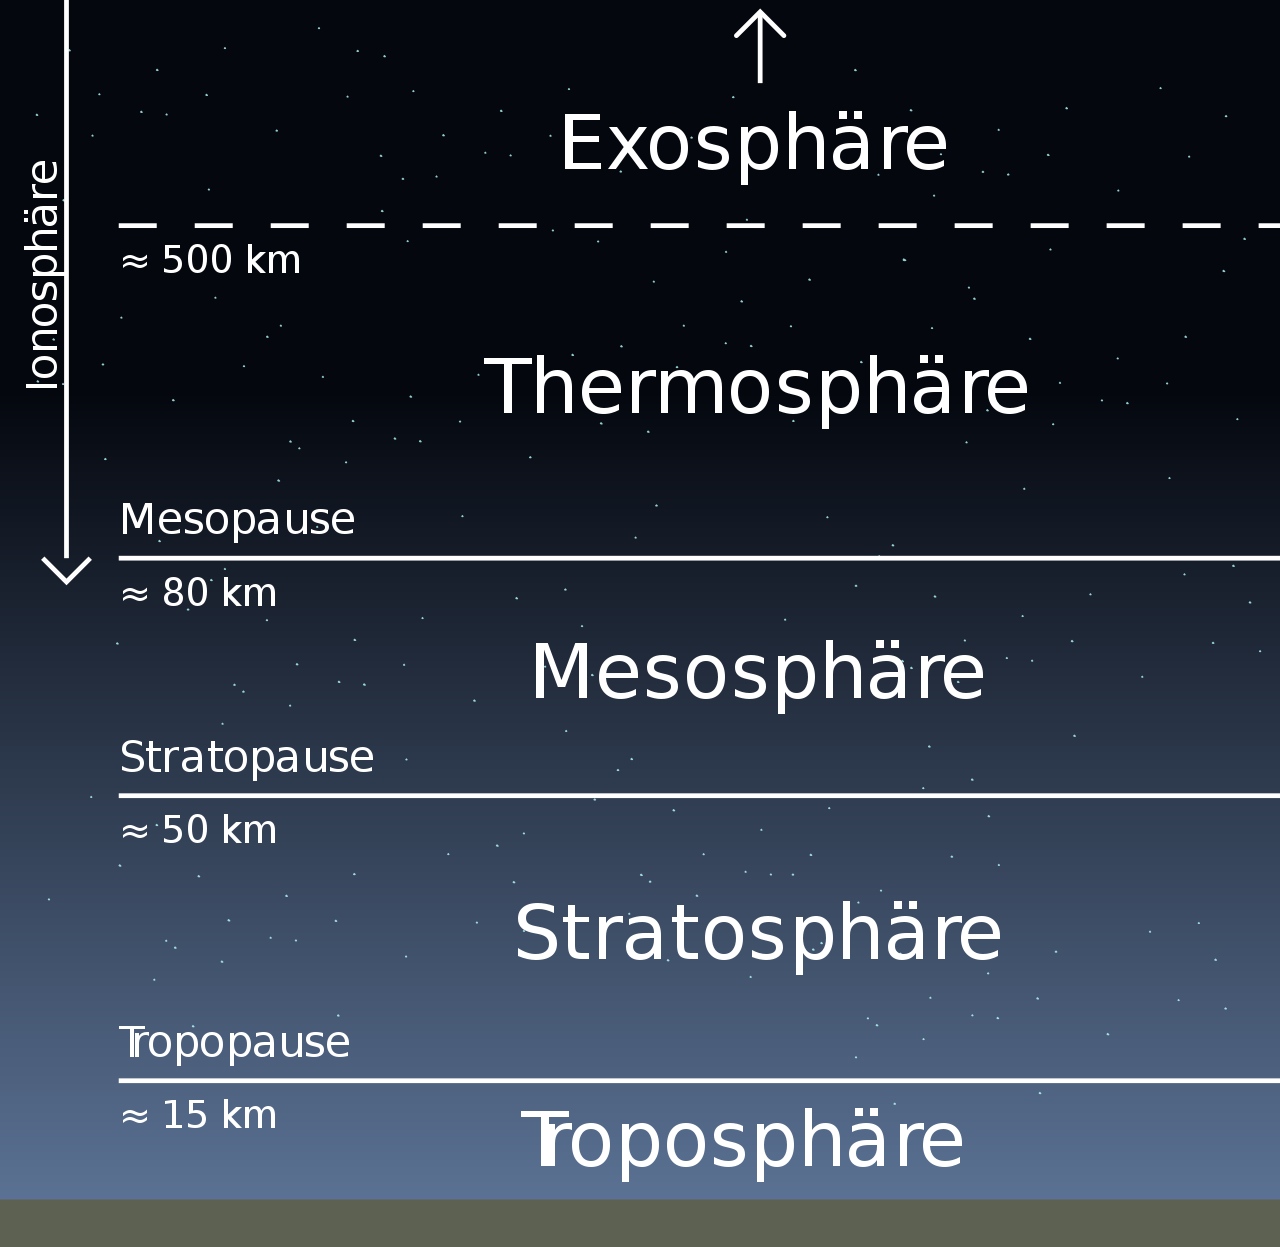
\includegraphics[width=\textwidth]{fig/photo/erdatmosphäre.png}
        \caption{Schichten der Atmosphäre \cite{amt_zones}}
    \end{figure}
    \end{columns}
\end{frame}

\begin{frame}
    \frametitle{Inhaltsangabe}
    \begin{itemize}
        \item[-] Theoretische Grundlagen
    \vfill
		\item[-] Labormessungen
    \vfill
		\item[-] Atmosphärische Messungen 
	\end{itemize}
\end{frame}

\begin{frame}
    \frametitle{DOAS}
    \section{Theoretische Grundlagen}
    \begin{columns}

      \column{0.5\textwidth}
        \begin{figure}
        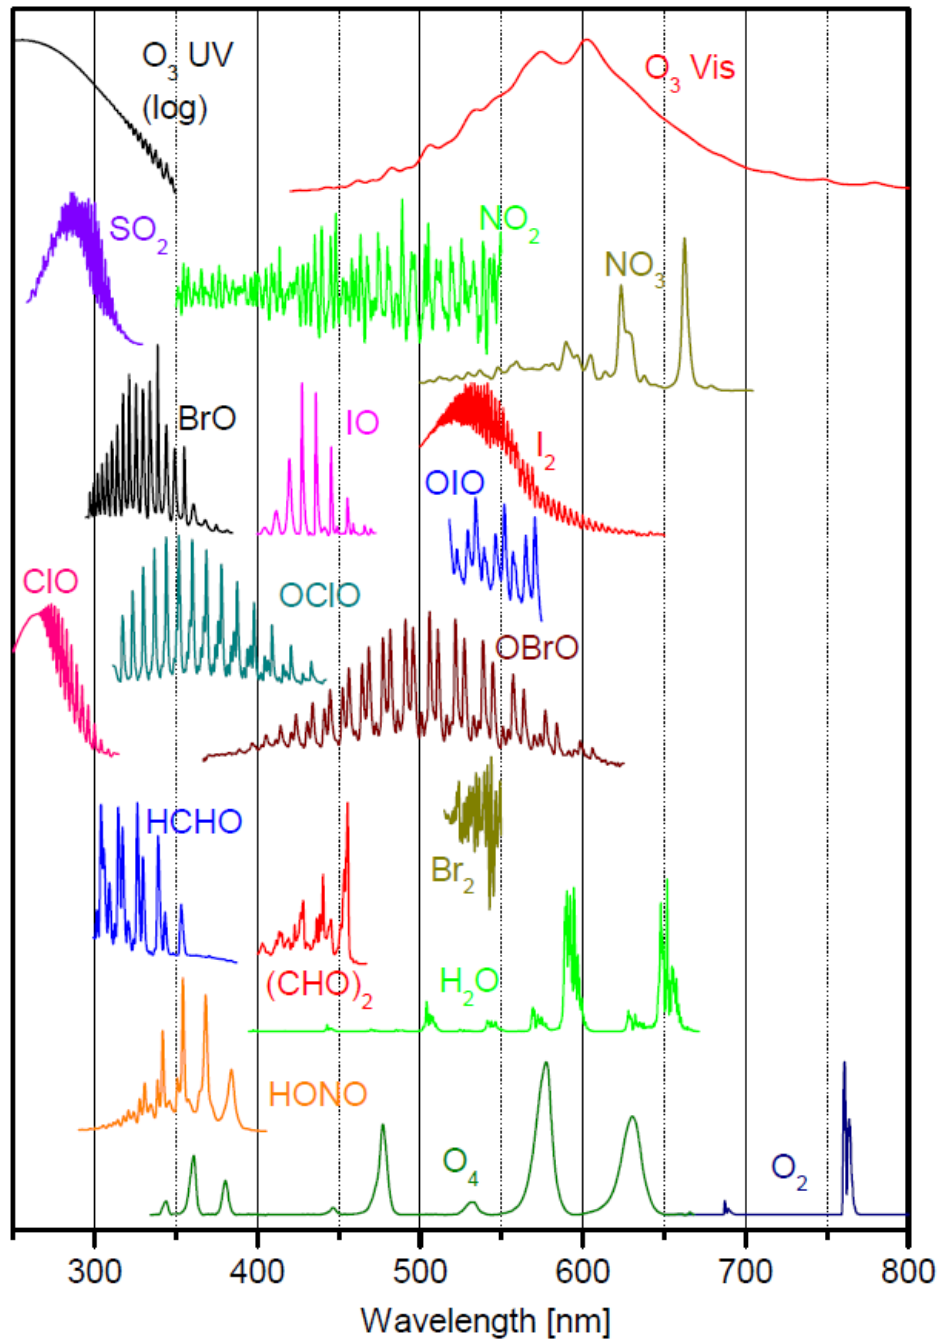
\includegraphics[width=0.8\textwidth]{fig/gas_spectra.png}
        \caption{Charakteristische Absorptionsstrukturen \cite{atm_script}}
        \end{figure}
    
      \column{.5\textwidth}
    	\begin{itemize}
        	\item[-] Verwendung: Vorkommen von Spurengasen in Tropo- und Stratosphäre
        	\item[-] Benutze charakteristische Absorptionsstrukturen von Molekülen
        	\item[-] Vergleich von optischen Dichten
    	\end{itemize}
	\end{columns}
\end{frame}

\begin{frame}
\frametitle{Messgrößen}
\begin{itemize}
    \item[-] Konzentration: Moleküle pro Volumeneinheit
        \pause
    \item[-] Säulendichte: $CD = \int \rho (s) \dd s$
        \begin{itemize}
            \item schräge Säulendichte SCD oder $S$
            \item vertikale Säulendichte VCD
            \item werden in $\frac{\text{Moleküle}}{\text{cm}^2}$ angegeben
            \item für \ch{O3}: $1 \text{Dobson Unit(DU)} = 2.6 \cdot 10^{16} \frac{\text{Moleküle}}{\text{cm}^2}$ 
        \end{itemize}
        \pause
    \item[-] Mischverhältnis: Relativer Anteil von Spurengas zu Luftmenge
    \end{itemize}
\end{frame}

\begin{frame}
    \frametitle{Lambert-Beer Gesetz}
    \begin{figure}[h]
        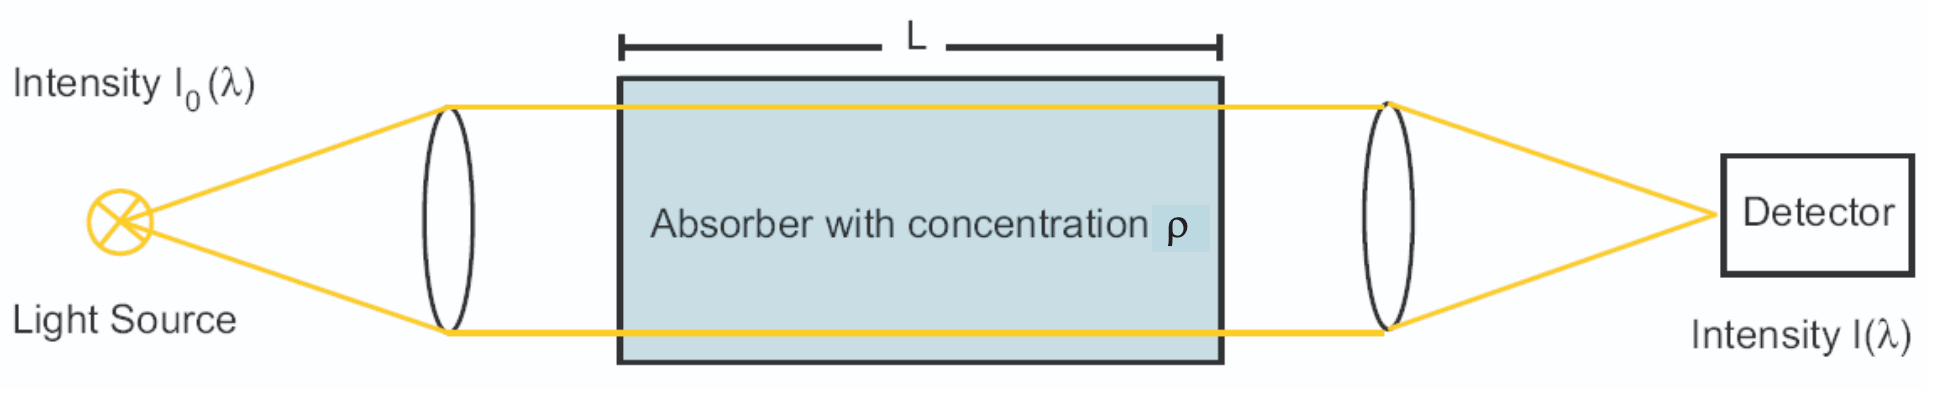
\includegraphics[width=0.8\textwidth]{fig/lambert_beer.png}
        \caption{Absorption eines Lichtstrahles \cite{atm_script}}
    \end{figure}
    \begin{align}
    	I(\lambda, L) = I_0 (\lambda) \exp (- \rho  L \sigma (\lambda) )
    \end{align}
    \begin{itemize}
        \item $L$ Länge des Mediums
        \item $\rho$ Dichte
        \item $\sigma (\lambda)$ Absorptionswirkungsquerschnitt % Absorptionswirkungsquerschnitt ist wahrscheinlichkeit dass bei bestimmen winkel absorption stattfindet
    \end{itemize}
\end{frame}

\begin{frame}
    \frametitle{DOAS-Fit}
    Forme Lambert-Beer um:
	\begin{align}
        & I = I_0 \exp (-\rho L \sigma (\lambda)) \\
        \Leftrightarrow \ &\tau = \log \frac{I}{I_0} = - \rho L \sigma (\lambda).
	\end{align}
    \pause
	Erstelle Fit durch Minimierung von
    \begin{align}
        \chi^2 = ( \log \frac{I_0}{I} -\underbrace{\rho L}_{\text{CD}} \sigma )^2. 
    \end{align}
\end{frame}

\begin{frame}
    \frametitle{Kurzbandeffekte}
    \begin{columns}
      \column{0.6\linewidth}
    	\begin{figure}
        	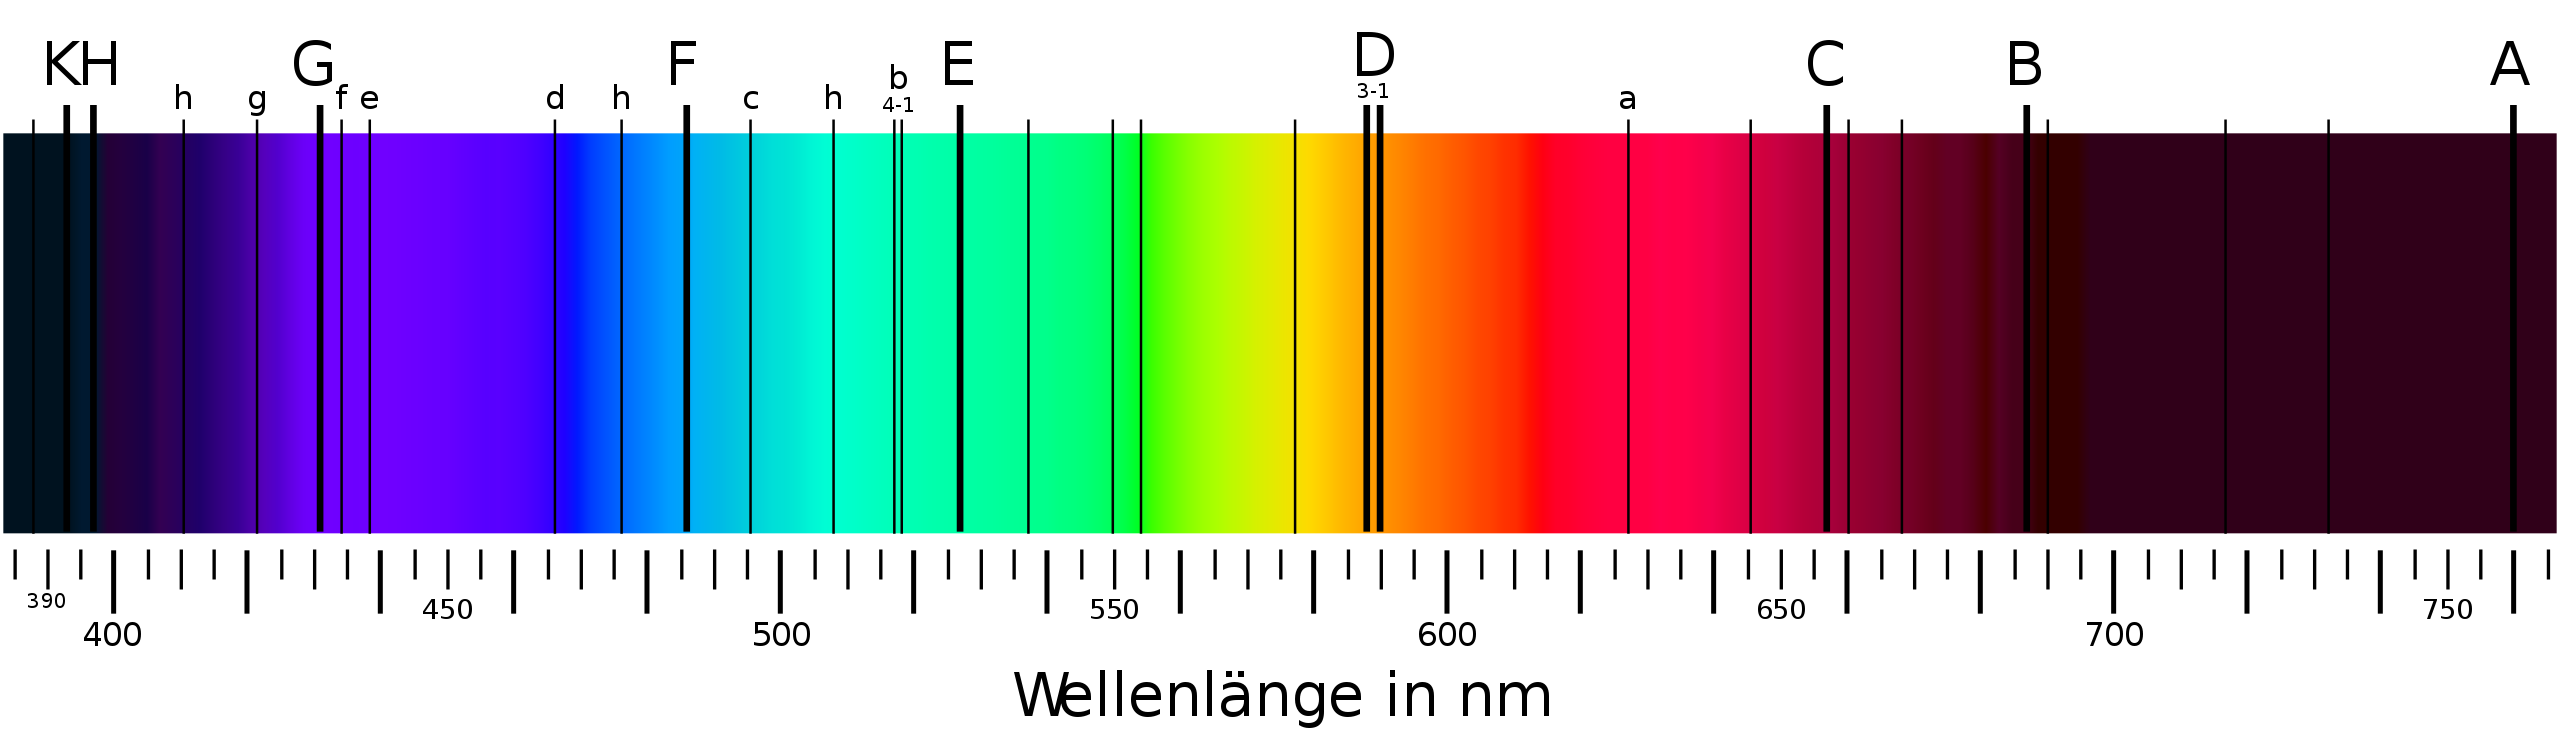
\includegraphics[width=\textwidth]{fig/fraunhofer_linien.png}
        	\caption{Fraunhoferspektrum \cite{fraunhofer}}
    	\end{figure}
      \column{0.4\linewidth}
        \begin{itemize}
			\item[-]{Fraunhoferlinien}
        	\pause
        	\item[-]{Ring-Effekt}
        \end{itemize}
    \end{columns}
\end{frame}

\begin{frame}
    \frametitle{Breitbandeffekte}
    \begin{itemize}
        \item[-] Elastische Streuung von Sonnenlicht $\to$ Mie und Rayleigh Streuung
            \pause
        \item[-] Summe aus Streuung und Absorption : \textit{Extinktion} $\epsilon_M$ und $\epsilon_R$
            \pause
    Rayleigh: $\sim \lambda^{-4}$\\
    Mie: keine starke $\lambda$ Abhängigkeit
    \end{itemize}
\end{frame}

\begin{frame}
    \frametitle{Atmosphärische Effekte}
    \begin{figure}
    	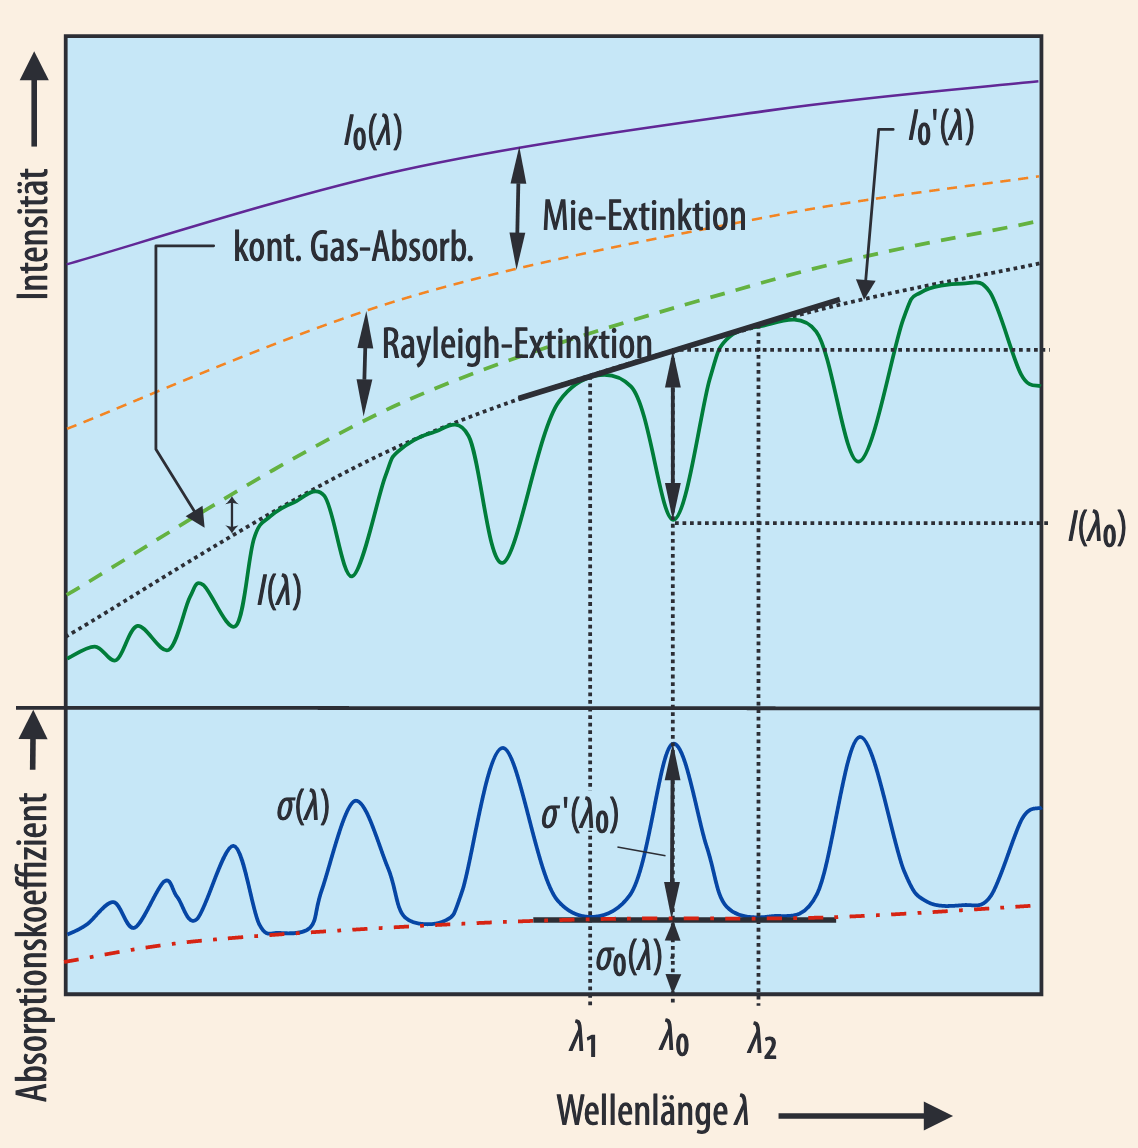
\includegraphics[width=0.65\linewidth]{fig/rayleigh_mie.png}
    	\caption{Breit- und Kurzbandeffekte \cite{platt10}}
    \end{figure}
\end{frame}

\begin{frame}
    \frametitle{Modifiziertes Lambert-Beer Gesetz}
    \begin{align}
        I = I_0 \exp(-R - \sum_i \sigma_i S_i) \exp\left( -L (\sigma_{i0}\rho_0) + \epsilon_R + \epsilon_M\right)
    \end{align}
    Erste Exponentialfunktion: Kurzbandeffekte\\
    Zweite Exponentialfunktion: Breitbandeffekte\\
    \pause
    Neues $\chi^2$:
    \begin{align}
        \chi^2 = \left( \log\frac{I_0 + I_\text{Ofs}}{I} - R - \sum_i \sigma_i S_i - \sum_k b_k \lambda^k \right)^2
    \end{align}
\end{frame}

\begin{frame}
    \section{Auflösung des Spektrometers}
    \frametitle{Messung mit Quecksilberdampflampe}
    \begin{columns}
      \column{0.4\linewidth}
    	\begin{figure}
        	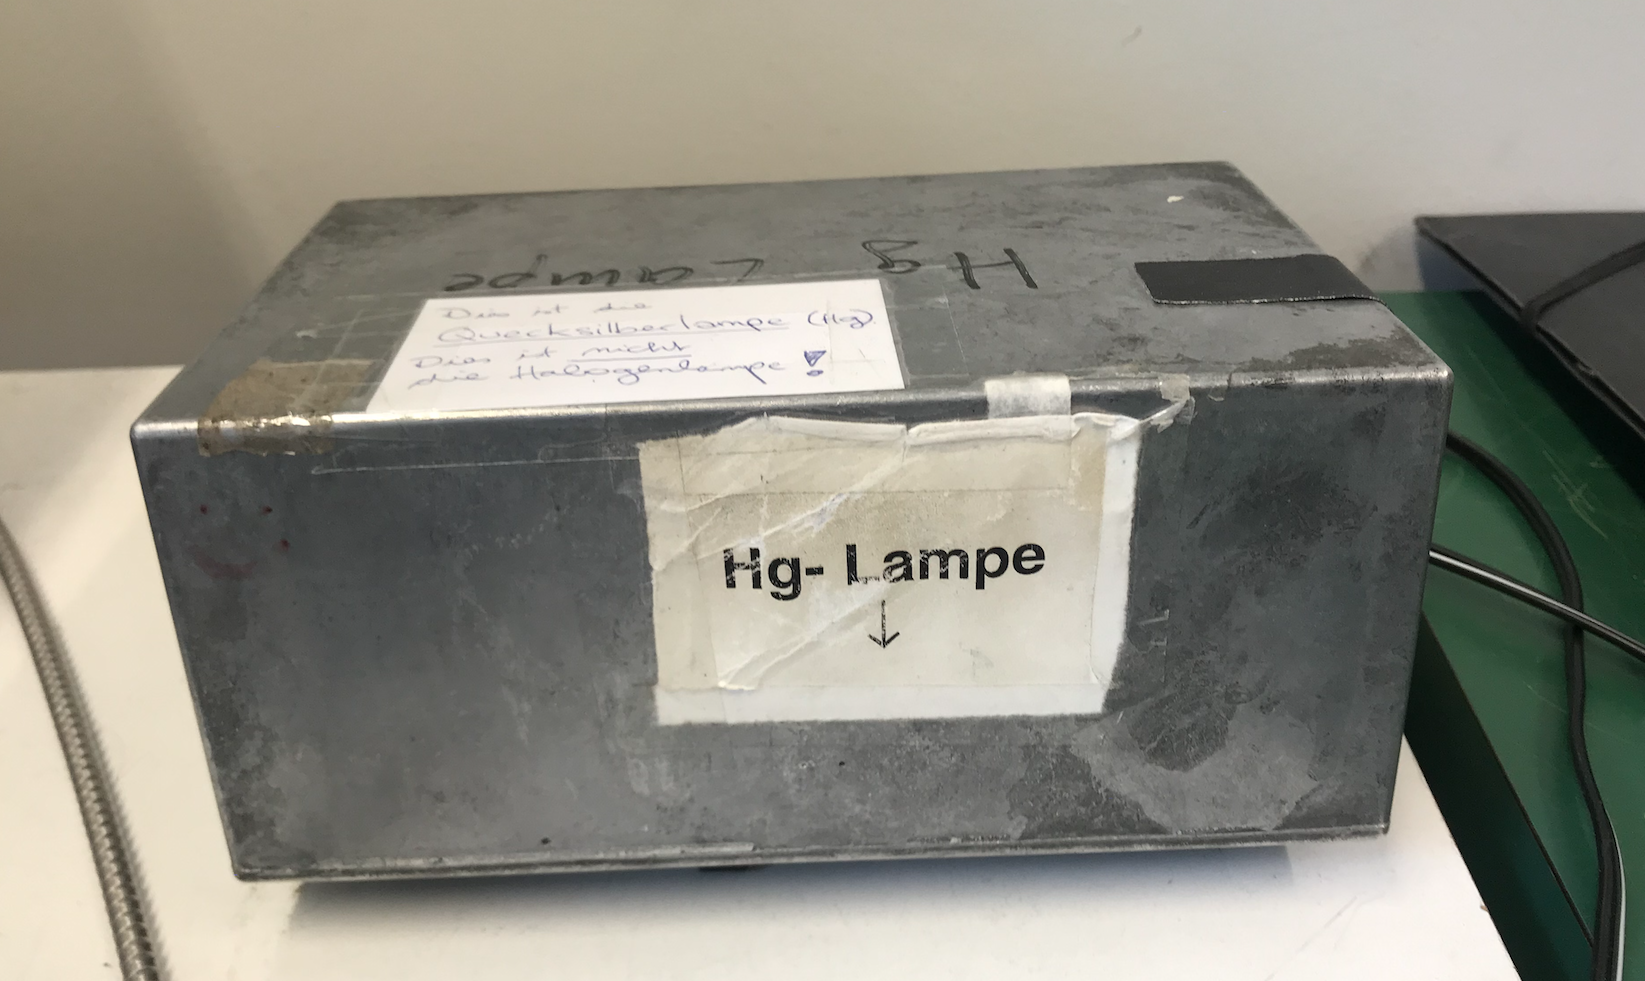
\includegraphics[width=\textwidth]{fig/photo/hg_lampe.png}
        	\caption{Verwendete Lichtquelle}
    	\end{figure}
      \column{0.6\linewidth}
		\begin{figure}
        	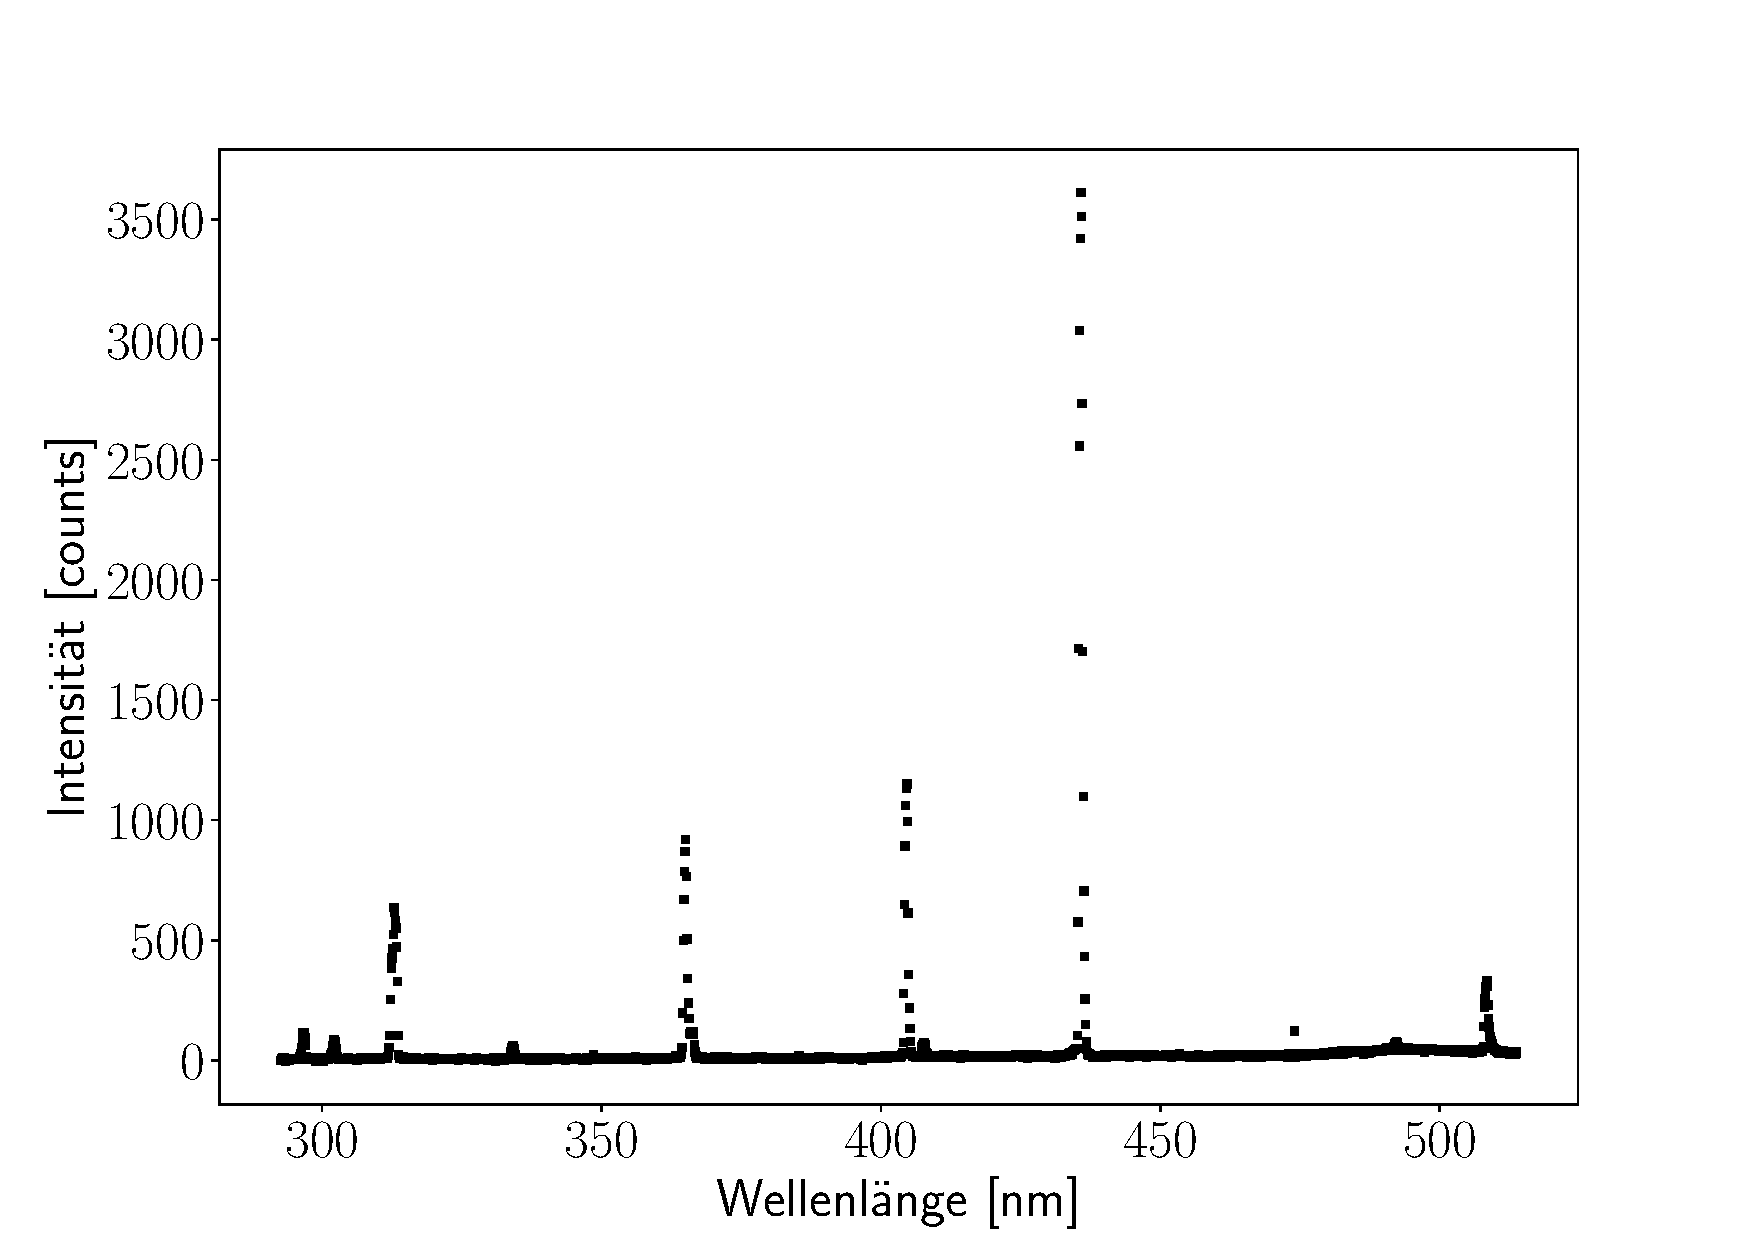
\includegraphics[width=\textwidth]{fig/hg_spectrum.pdf}
        	\caption{Spektrum der Quecksilberdampflampe}
    	\end{figure}
    \end{columns}
\end{frame}

\begin{frame}
    \frametitle{Auflösung des Spektrometers} 
    \begin{tabular*}{\linewidth}{@{\extracolsep{\fill}} c c c}
    	\toprule
    	Maximum & Wellenlänge & FWHM [\si{nm}] \\
    	\midrule
    	1 & $\sim 313$ & $1.2 \pm 0.1$ \\
    	2 & $\sim 365$ & $0.8 \pm 0.1$ \\
    	3 & $\sim 404$ & $0.6 \pm 0.1$ \\
    	4 & $\sim 436$ & $0.7 \pm 0.1$ \\
    	\bottomrule
	\end{tabular*}
    \captionof{figure}{FWHM der Intensitätsmaxima}
\end{frame}

\begin{frame}
    \section{Labormessungen}
    \frametitle{Halogenlampenmessung (\textit{aktiv} DOAS)}

    \begin{figure}[h]
        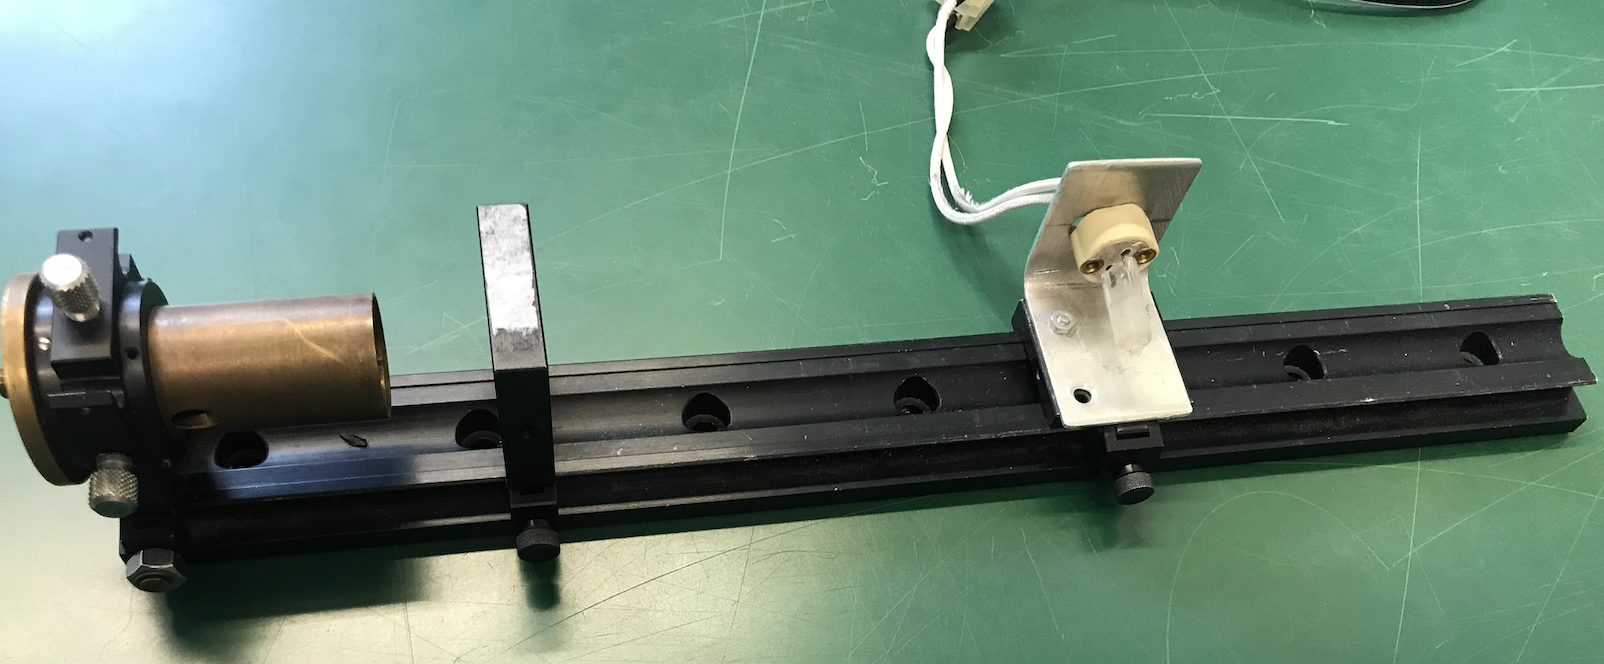
\includegraphics[width=0.7\textwidth]{fig/photo/aufbau_1.png}
    \end{figure}
	\vspace{-0.2cm}
    \begin{figure}[h]
        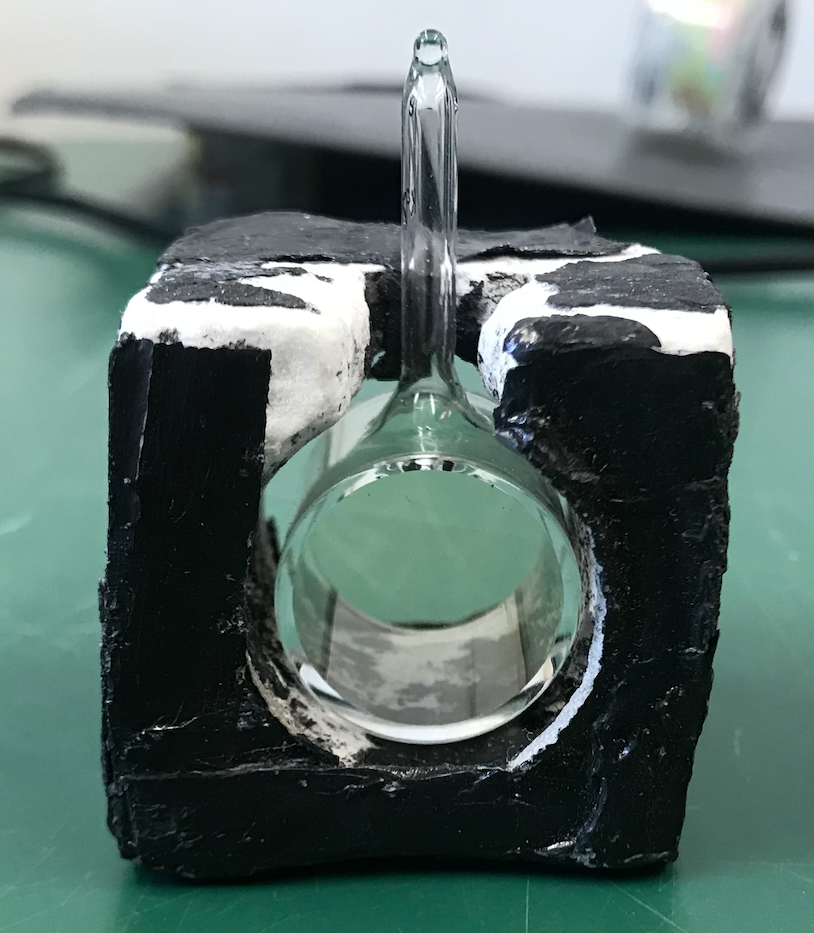
\includegraphics[width=0.3\textwidth]{fig/photo/glas_test.png}
        \caption{Versuchsaufbau Labormessung}
    \end{figure}
\end{frame}

\begin{frame} 
    \frametitle{Halogenlampenmessung}
    
	\begin{itemize}
    	\item Labormessung: atmosphärische Einflüsse vernachlässigbar
	\end{itemize}

	\begin{align}
	 	\to \tau = \sigma_{\ch{NO2}}(\lambda) \cdot \rho_{\ch{NO2}} \cdot L
	\end{align}
	
    \begin{itemize}
    	\item Fitbereich: Suche nach Überlagerung mit \ch{NO2} Referenz
	\end{itemize}

	\begin{figure}[h]
		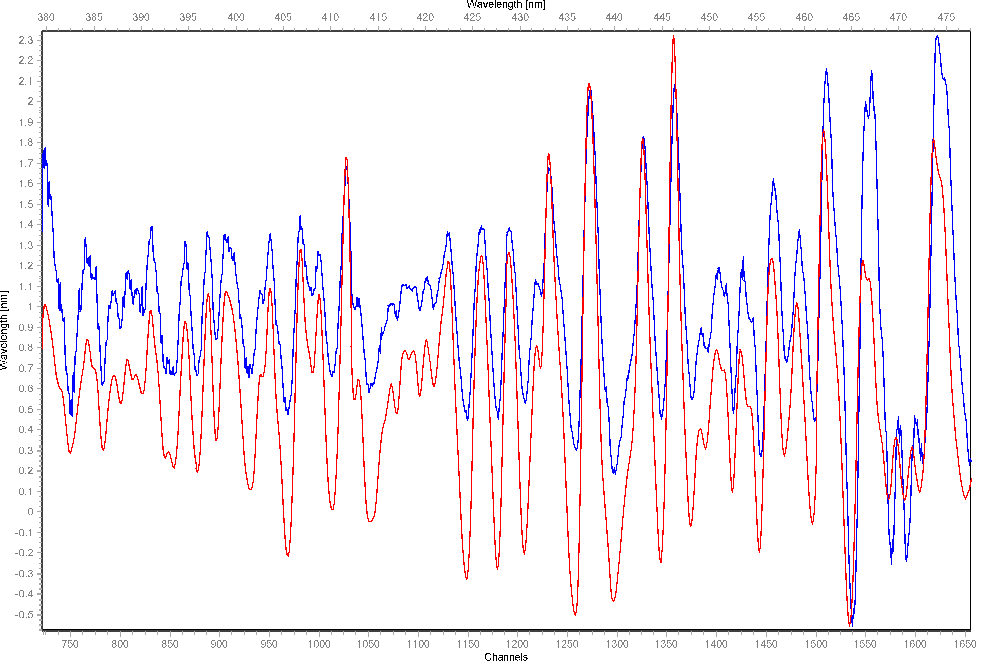
\includegraphics[width=0.5\textwidth]{fig/range_search_test.png}
		\caption{Vergleich der optischen Dichten von Literatur- und Versuchsspektrum}
	\end{figure}
\end{frame} 

\begin{frame}
	\frametitle{Halogenlampenmessung}
     \begin{figure}[h]
    	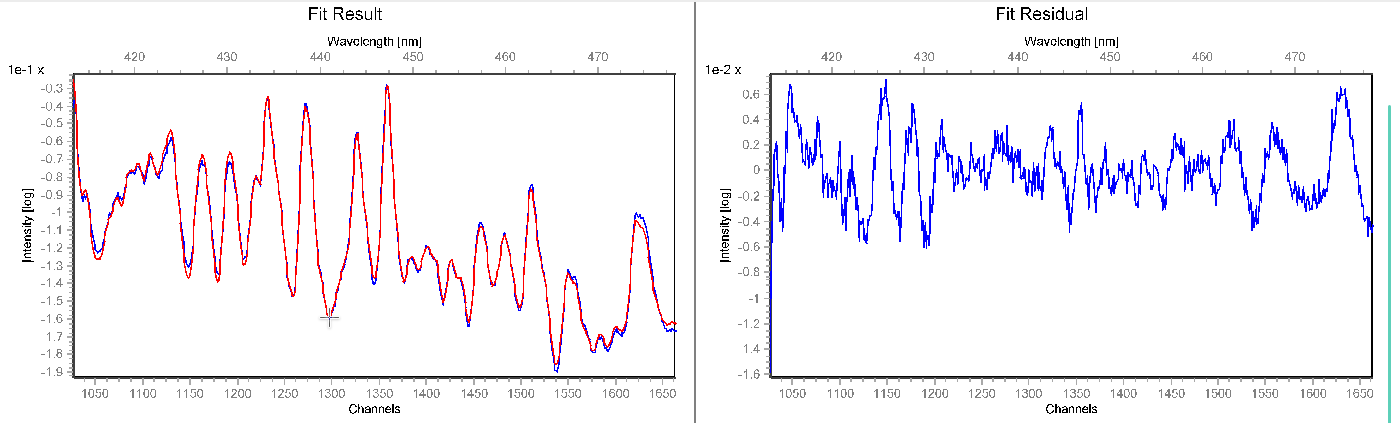
\includegraphics[width=1\textwidth]{fig/fit_labor.png}
    	\caption{Fitergebnis der \ch{NO2} Labormessung}
    \end{figure}

    \begin{itemize} 
    	\item Fitbereich: $(413.46 - 477.25) \si{nm}$
    	
    		\begin{align}
    		   \text{Fitparameter:}\ \chi^2 &= 4.367 \cdot 10^{-3}\\
    		   \text{fit coeff} &= 4.96 \cdot 10^{17} \pm 1.95 10^{15}
    		\end{align}
    		
    \end{itemize}
\end{frame} 

\begin{frame}
	\frametitle{Halogenlampenmessung}
	\begin{align}
		\text{Fitbereich:}\ (413.&46 - 477.25) \si{nm}\\
		\text{Fitparameter:}\ \chi^2 &= 4.367 \cdot 10^{-3}\\
		\text{fit coeff} &= 4.96 \cdot 10^{17} \pm 1.95 \cdot 10^{15}
	\end{align}
	
	\begin{align}    
		\to \rho_{\ch{NO2}} = (2.48 \pm 0.12) \cdot 10^{20} \si{\frac{\text{Moleküle}}{\ell}}
	\end{align}
\end{frame}

\begin{frame}
    \section{Atmosphärische Messungen}
    \frametitle{Atmosphärische Messungen (\textit{passiv} DOAS)}
    \begin{columns}
      \column{.5\textwidth}
    	\begin{figure}[h]
    		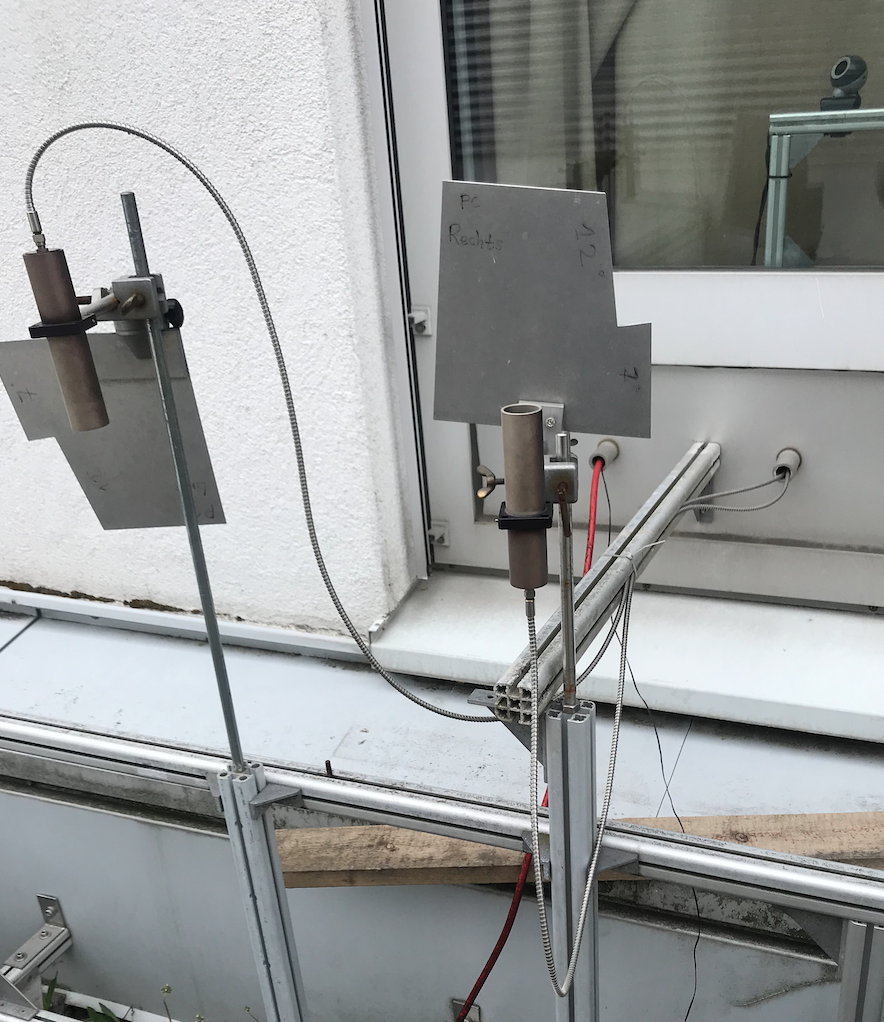
\includegraphics[width=1\textwidth]{fig/photo/aufbau_2.png}
    		\caption{Teleskopausrichtung}
    	\end{figure}
      \column{0.5\textwidth}
    	\begin{itemize}
    		\item[-] Jetzt erweitertes Lambert-Beer Gesetz
    		\item[-] Untersuchung von SCD
    	\end{itemize}
    \end{columns}
\end{frame}

\begin{frame}
    \frametitle{Tagesmessung \ch{NO2} und \ch{O3}}
	\begin{columns}
	  \column{0.5\textwidth}
	  	\begin{figure}
	  		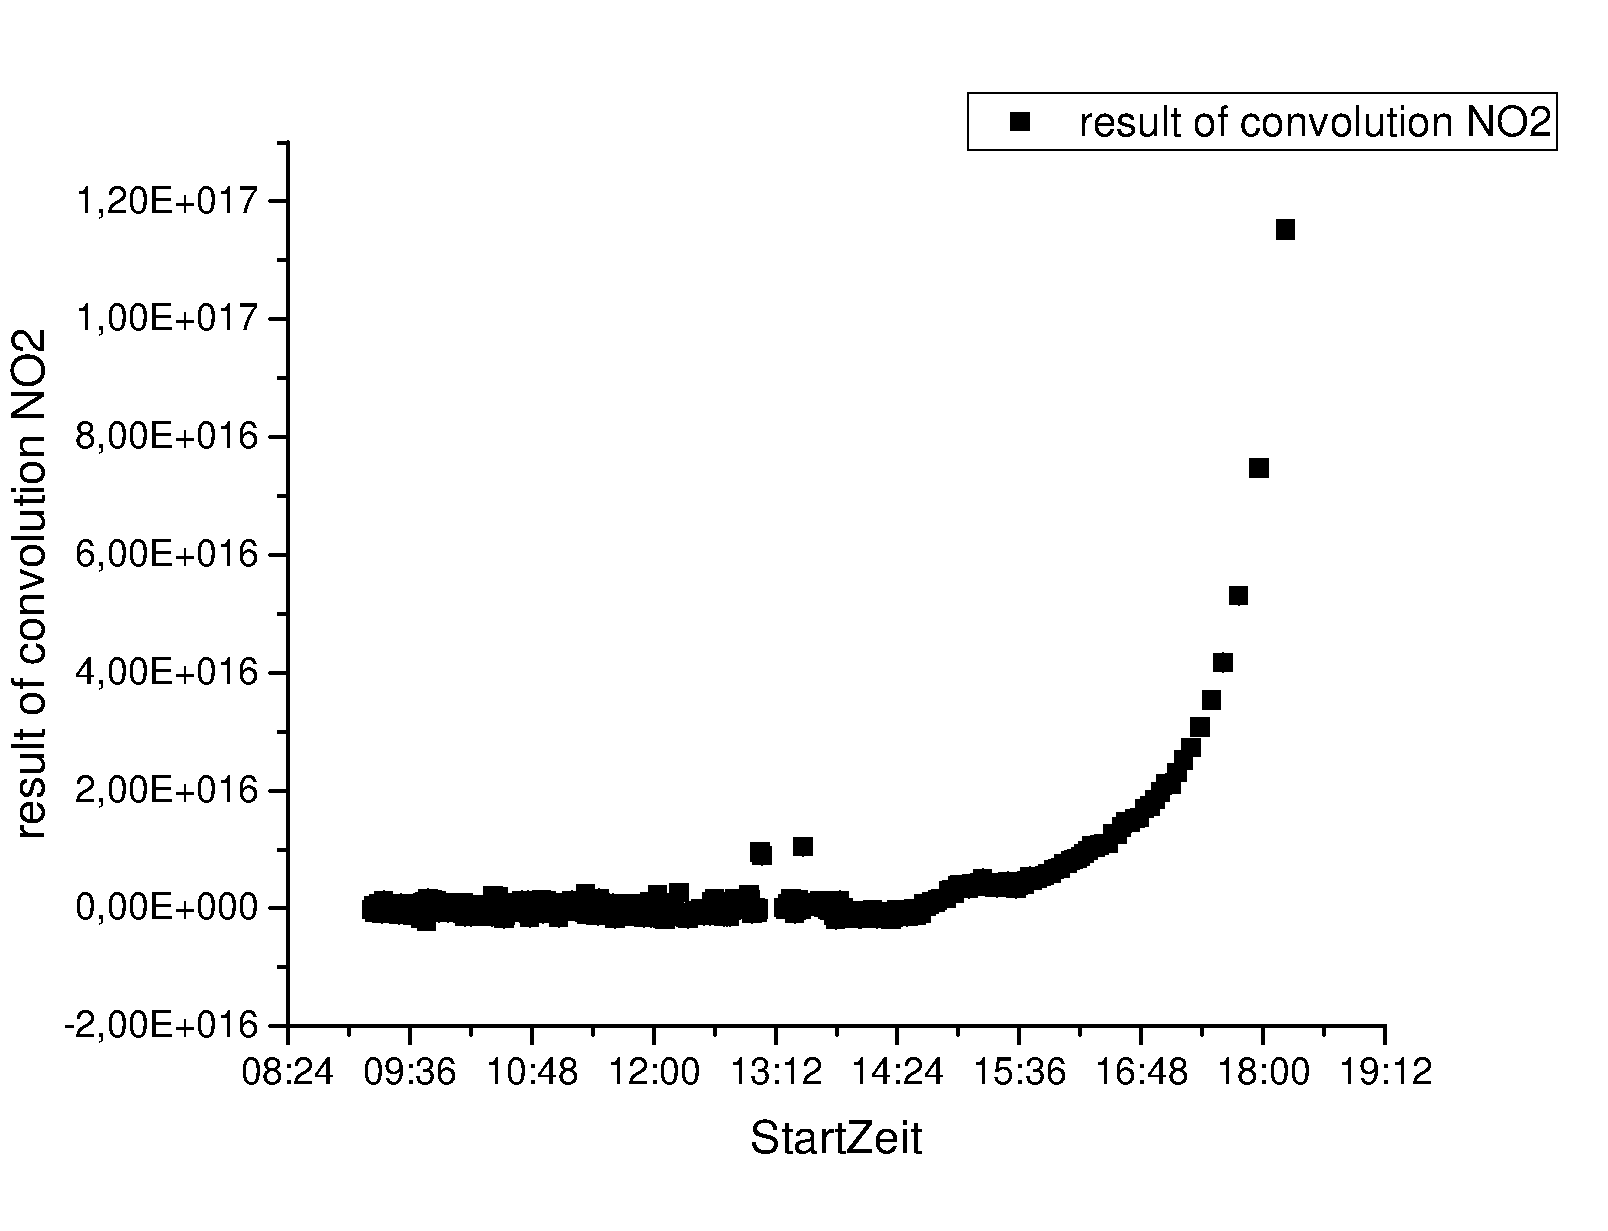
\includegraphics[width=1.2\linewidth]{fig/SCD_Time_Plot_NO2.pdf}
    		\caption{$\Delta \text{SCD}$ von \ch{NO2} über den Tag des 23.04.2019}
    		\label{fig:delta_SCD_time_NO2}
        \end{figure}
      \column{0.5\textwidth}
    	\begin{figure}
    		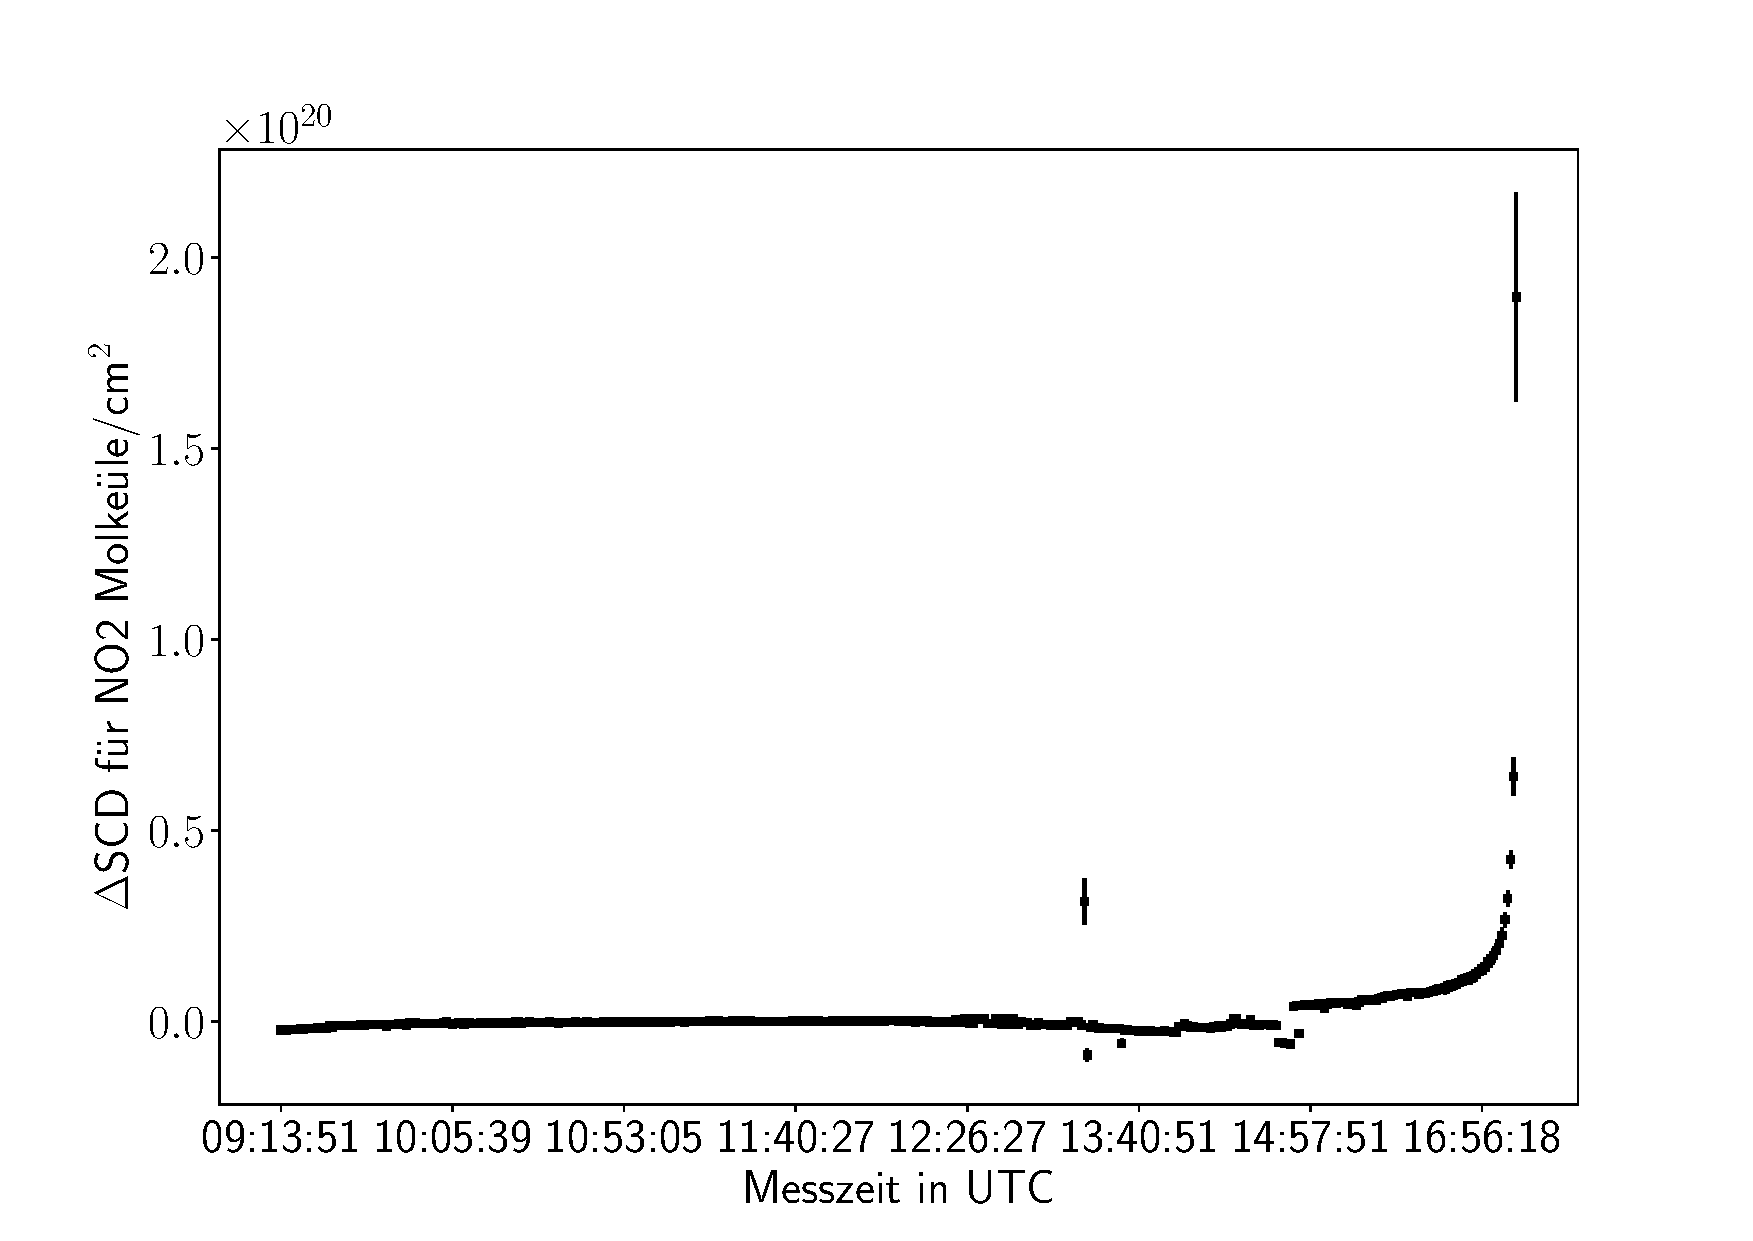
\includegraphics[width=1.2\linewidth]{fig/SCD_Time_Plot_O3.pdf}
    		\caption{$\Delta \text{SCD}$ von \ch{O3} über den Tag des 23.04.2019}
    		\label{fig:delta_SCD_time_O3}
    	\end{figure}  		
    \end{columns}
\end{frame}

\begin{frame}
    \frametitle{Tagesmessung \ch{NO2} und \ch{O3}}
    \begin{columns}
      \column{0.5\linewidth}    
    	Am Morgen:
    	\begin{align}
    		\ch{NO2} + h \nu \to \ch{NO} + \ch{O}(^3\text{P})
    	\end{align}
    \pause
    	Gleichzeitig Dissoziation:
    	\begin{align}
    		\ch{N2O5} + h \nu \to \ch{NO2} + \ch{NO3}
    	\end{align}
    \pause
    	Reagiert weiter:
    	\begin{align}
    		\ch{NO3} + h \nu \to \ch{NO} + \ch{O2}\\
    		\ch{NO3} + h \nu \to \ch{NO2} + \ch{O}
    	\end{align}
    \pause	
      \column{0.5\linewidth}
      	\ch{O3} und \ch{NO2} befinden sich im Gleichgewicht:
      		\begin{align}
      			\ch{O3} + \ch{NO} \rightleftharpoons \ch{NO2} + \ch{O2}
      		\end{align}
      	\ch{O3} hauptsächlich in der Stratosphäre	
    \end{columns}
\end{frame}

\begin{frame}
    \frametitle{Langley Plots}
    $\Delta$ SCD wird gegen Air Mass Factor (AMF) aufgetragen\\
    
    \begin{align}
        \text{AMF}(\theta) := \frac{\text{SCD}(\theta)}{\text{VCD}} \approx \frac{1}{\cos (\theta)}
    \end{align}
    
    \begin{figure}
        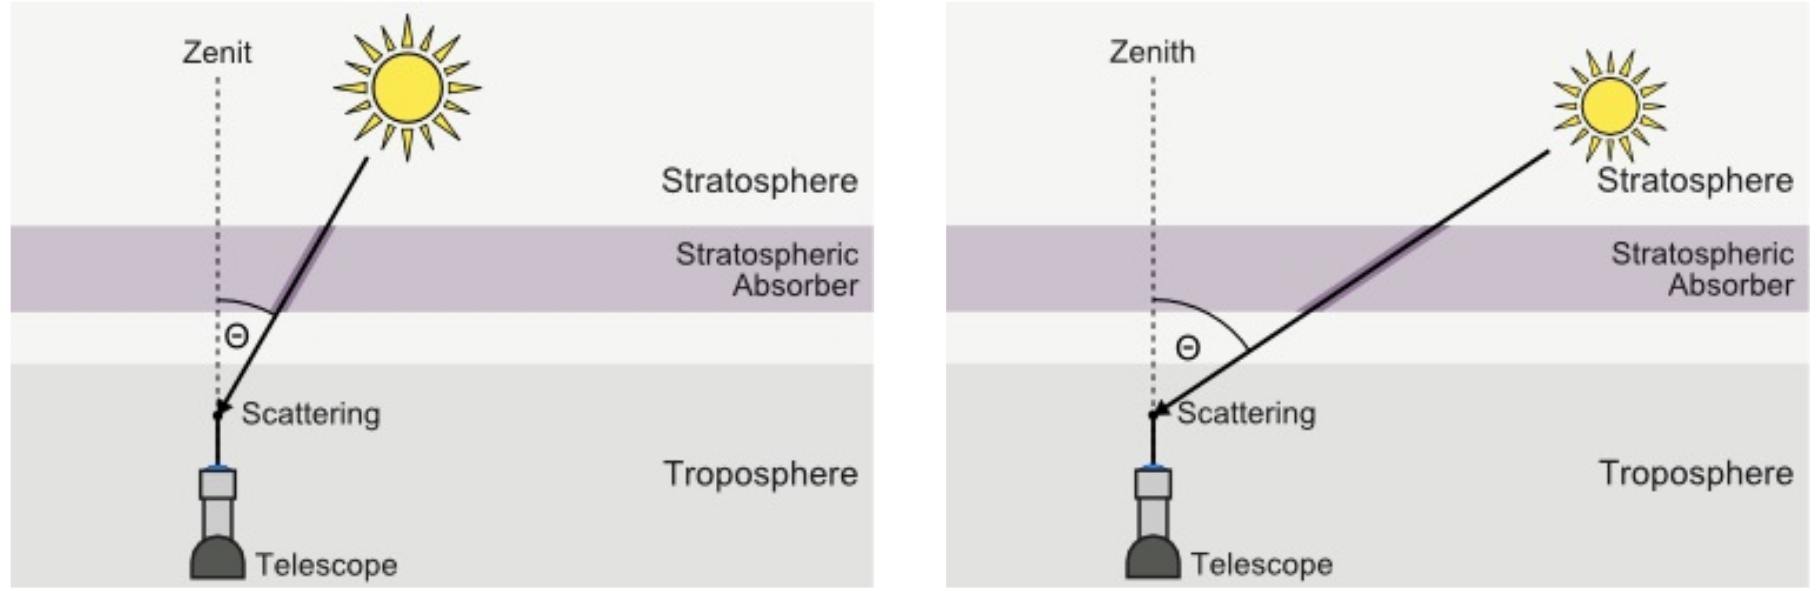
\includegraphics[width=0.9\linewidth]{fig/langley_sza.png}
        \caption{schematischer Lichtweg durch die Atmosphäre für unterschiedliche Sonnenzenitwinkel \cite{atm_script}}
    \end{figure}
\end{frame}

\begin{frame}
    \frametitle{Langley Plots}
    Die totale SCD ist $S = \Delta S + S_F$\\
    $S_F$ kann mit Langley Plot bestimmt werden\\
    Falls Konzentration konstant $\to$ Linearität im Langley Plot
    
    \begin{align}
    	\Delta \text{SCD}(AMF(\theta)) = \text{SCD}(AMF(\theta)) - S_F
    \end{align}
\end{frame}

\begin{frame}
    \frametitle{Langley Plot von \ch{NO2} und \ch{O3}}
    \begin{columns}
      \column{0.5\linewidth}
    	\begin{figure}
    		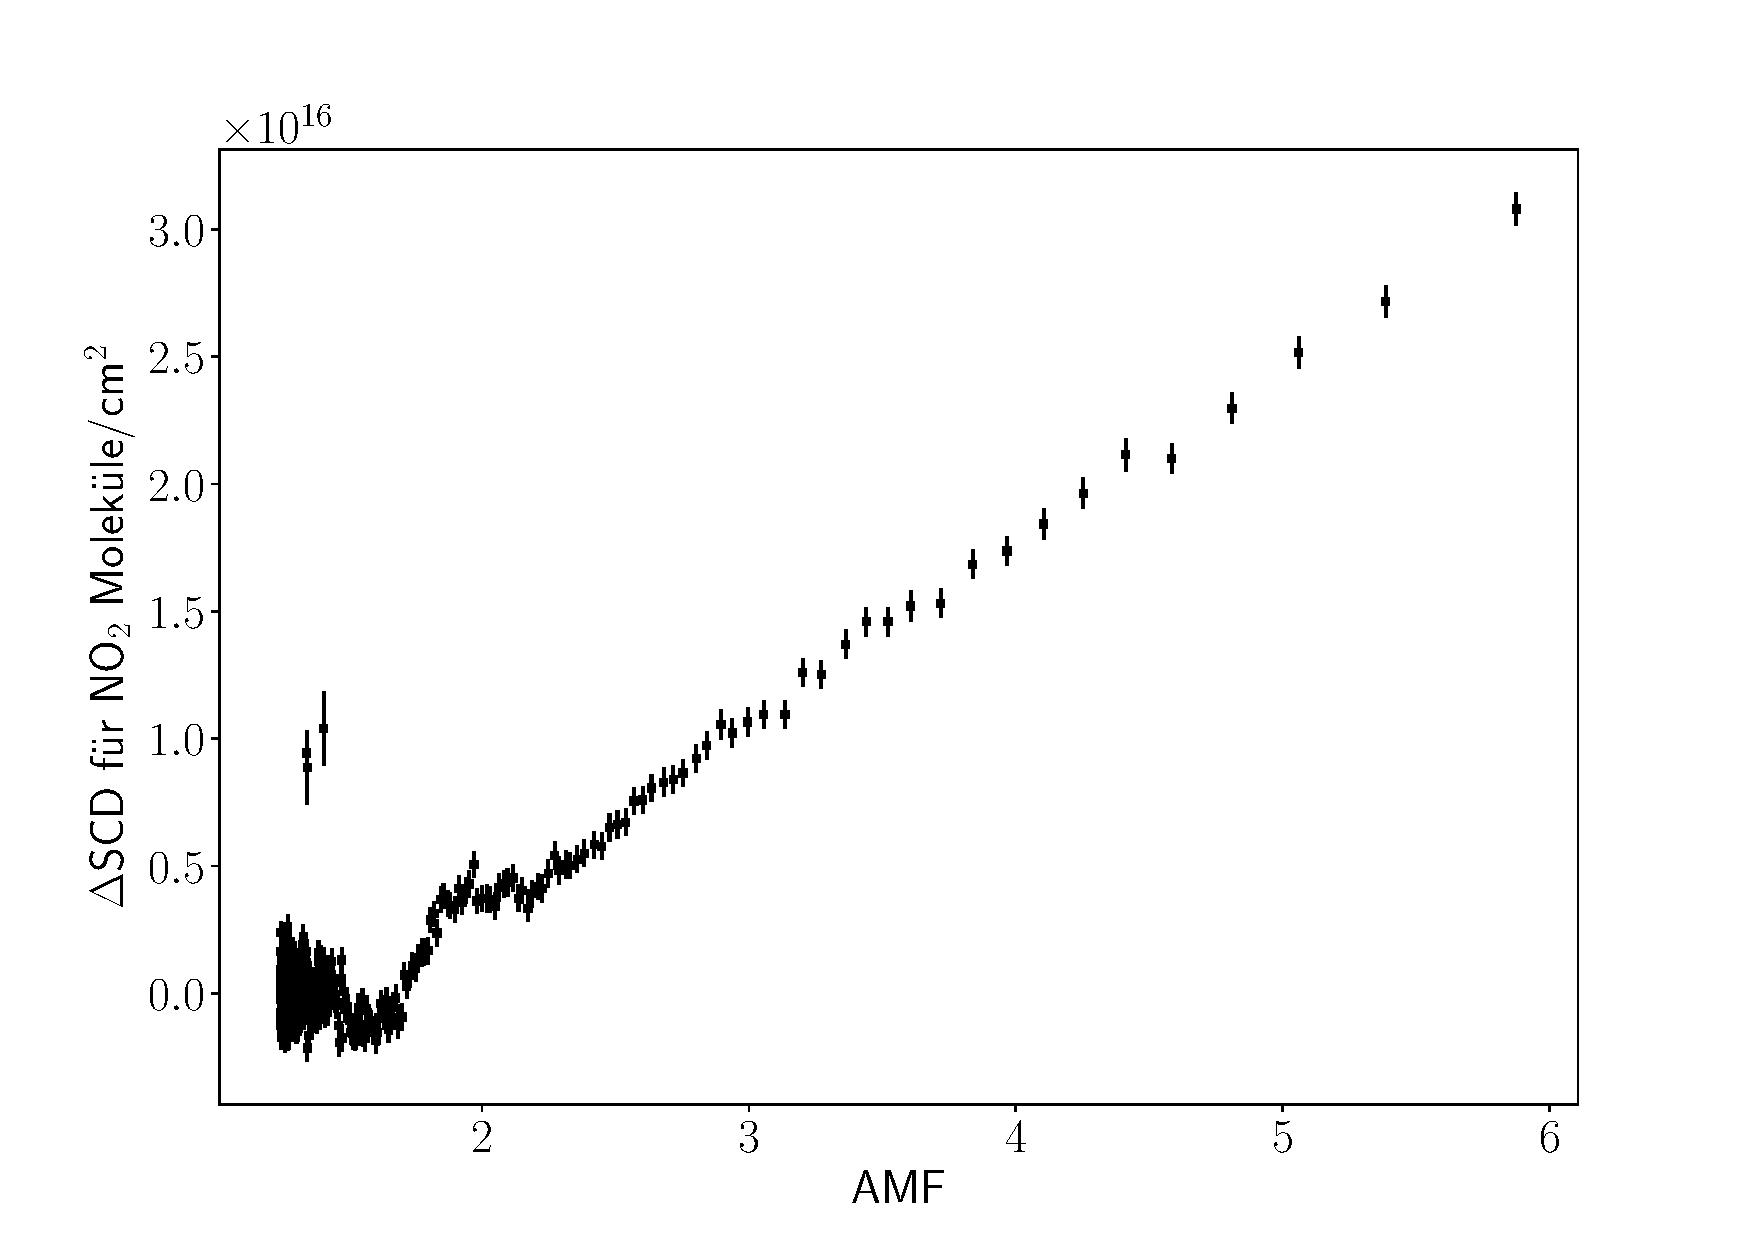
\includegraphics[width=1.15\linewidth]{fig/Langley_Plot_NO2_cut.pdf}
            \caption{Langley Plot von \ch{NO2}}   
	 	\end{figure}
 	  \column{0.5\linewidth}
 	    \begin{figure}
 	    	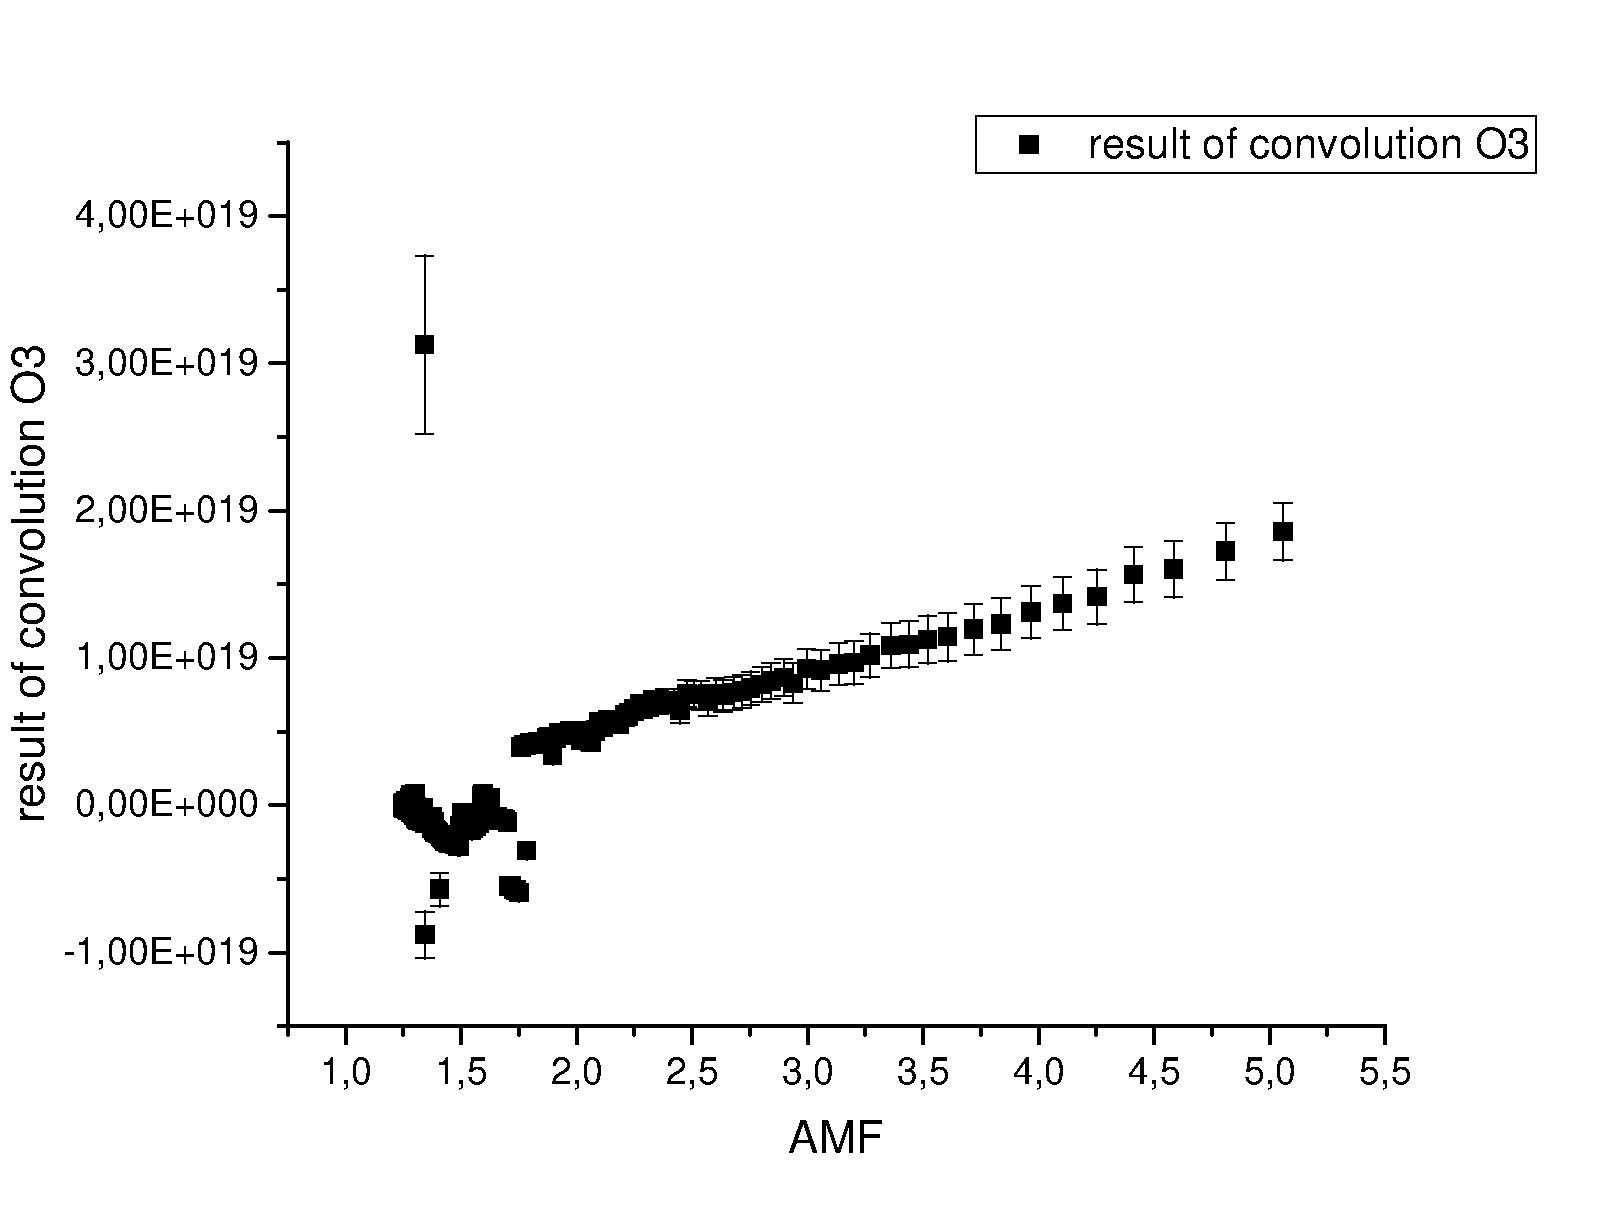
\includegraphics[width=1.15\linewidth]{fig/Langley_Plot_O3_cut.pdf}
 	        \caption{Langley Plot von \ch{O3}}
     	\end{figure} 
    \end{columns} 	
\end{frame}

\begin{frame}
    \frametitle{Fit $\Delta$SCD von \ch{O3}}
    \begin{figure}
    	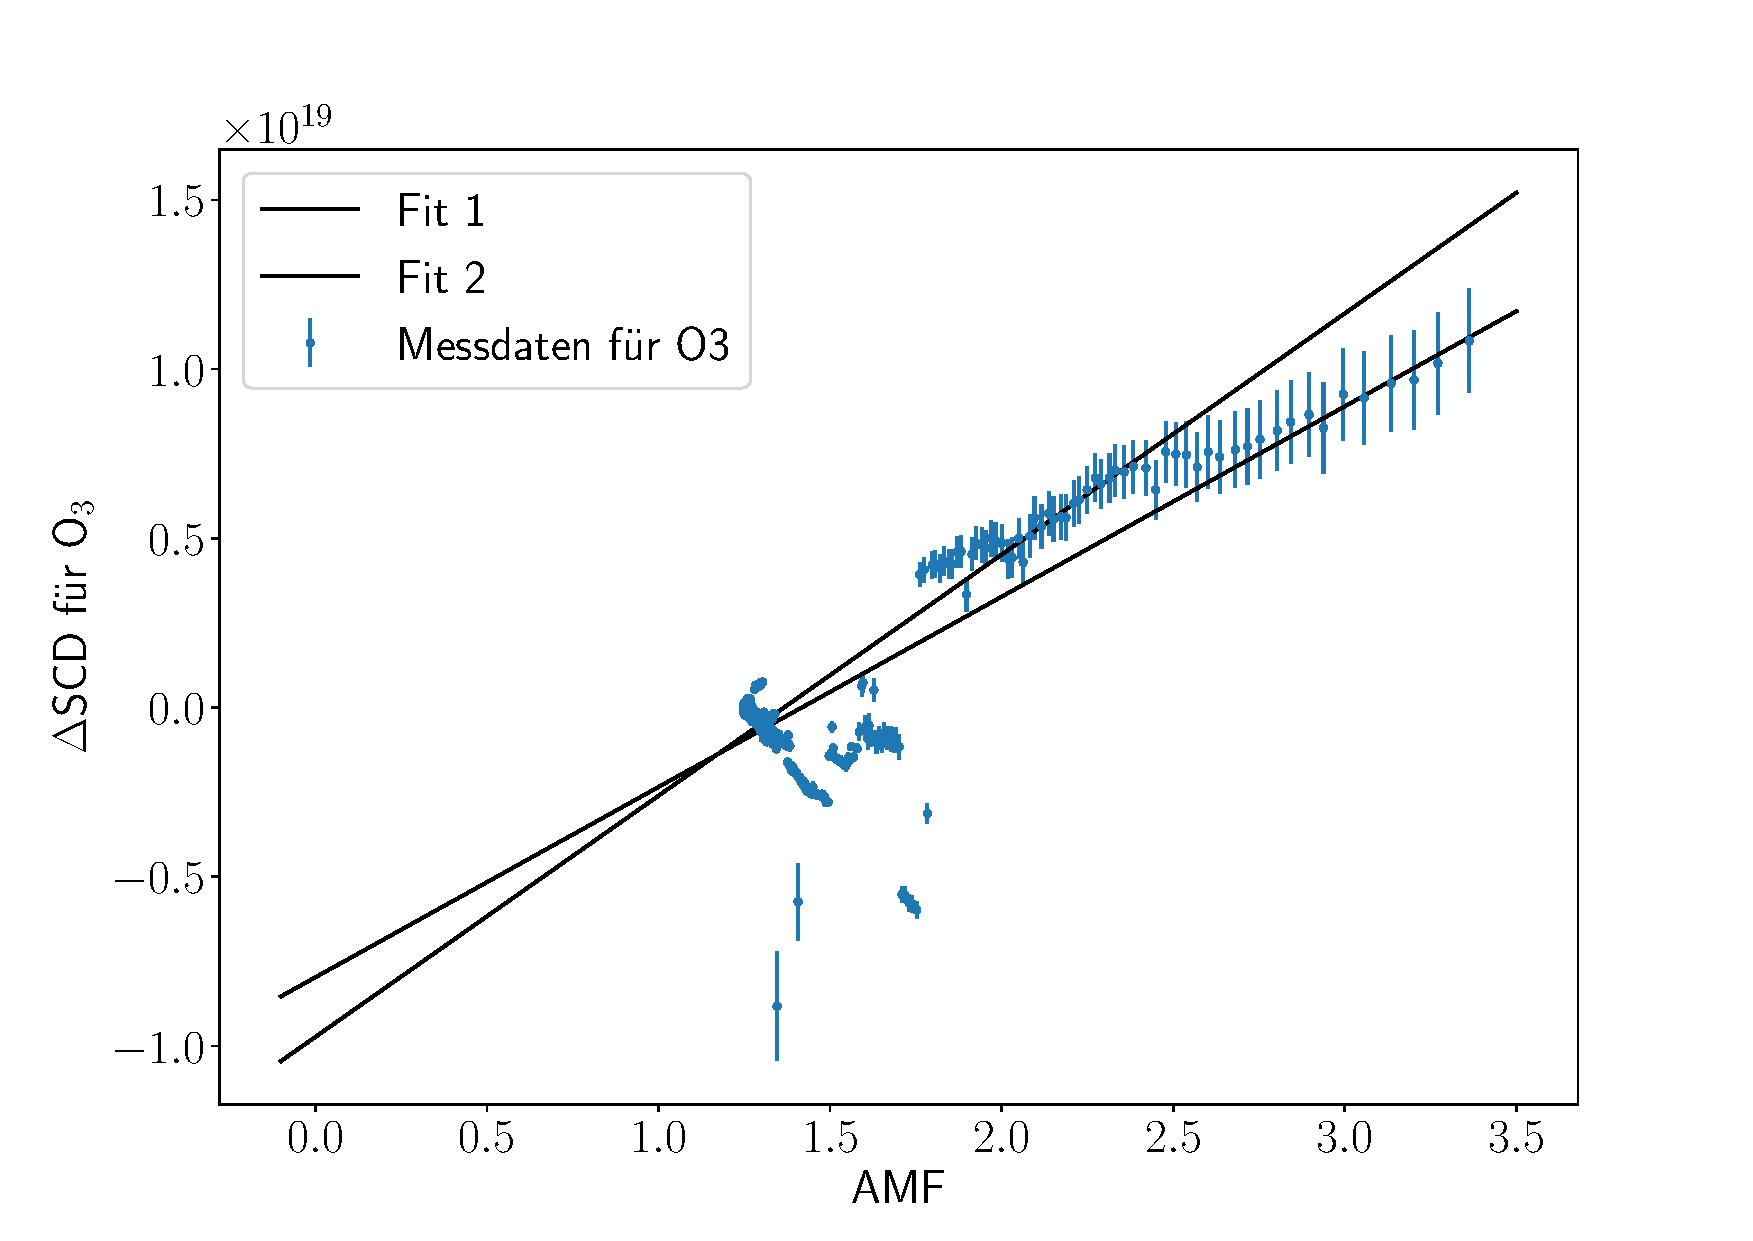
\includegraphics[width=.7\linewidth]{fig/scd_fit_o3.pdf}
    	\caption{Fit der Tagesmessung \ch{O3}}
    \end{figure}

	\begin{align}
		S_{ref}= (0.97 \cdot 10^{19}\pm 0.17 \cdot 10^{19}) \si{\frac{Moleküle}{cm^2}}
	\end{align}
\end{frame}

\begin{frame}
    \frametitle{Vertikale Säulendichte \ch{O3}}
    \begin{align}
    	\text{Vertikale Säulendichte (VCA) ist:}\	\text{VCD} = \text{SCD}_\text{ges} \cos (\theta)
    \end{align}
    
    \vspace{-1cm}
    
    \begin{figure}
    	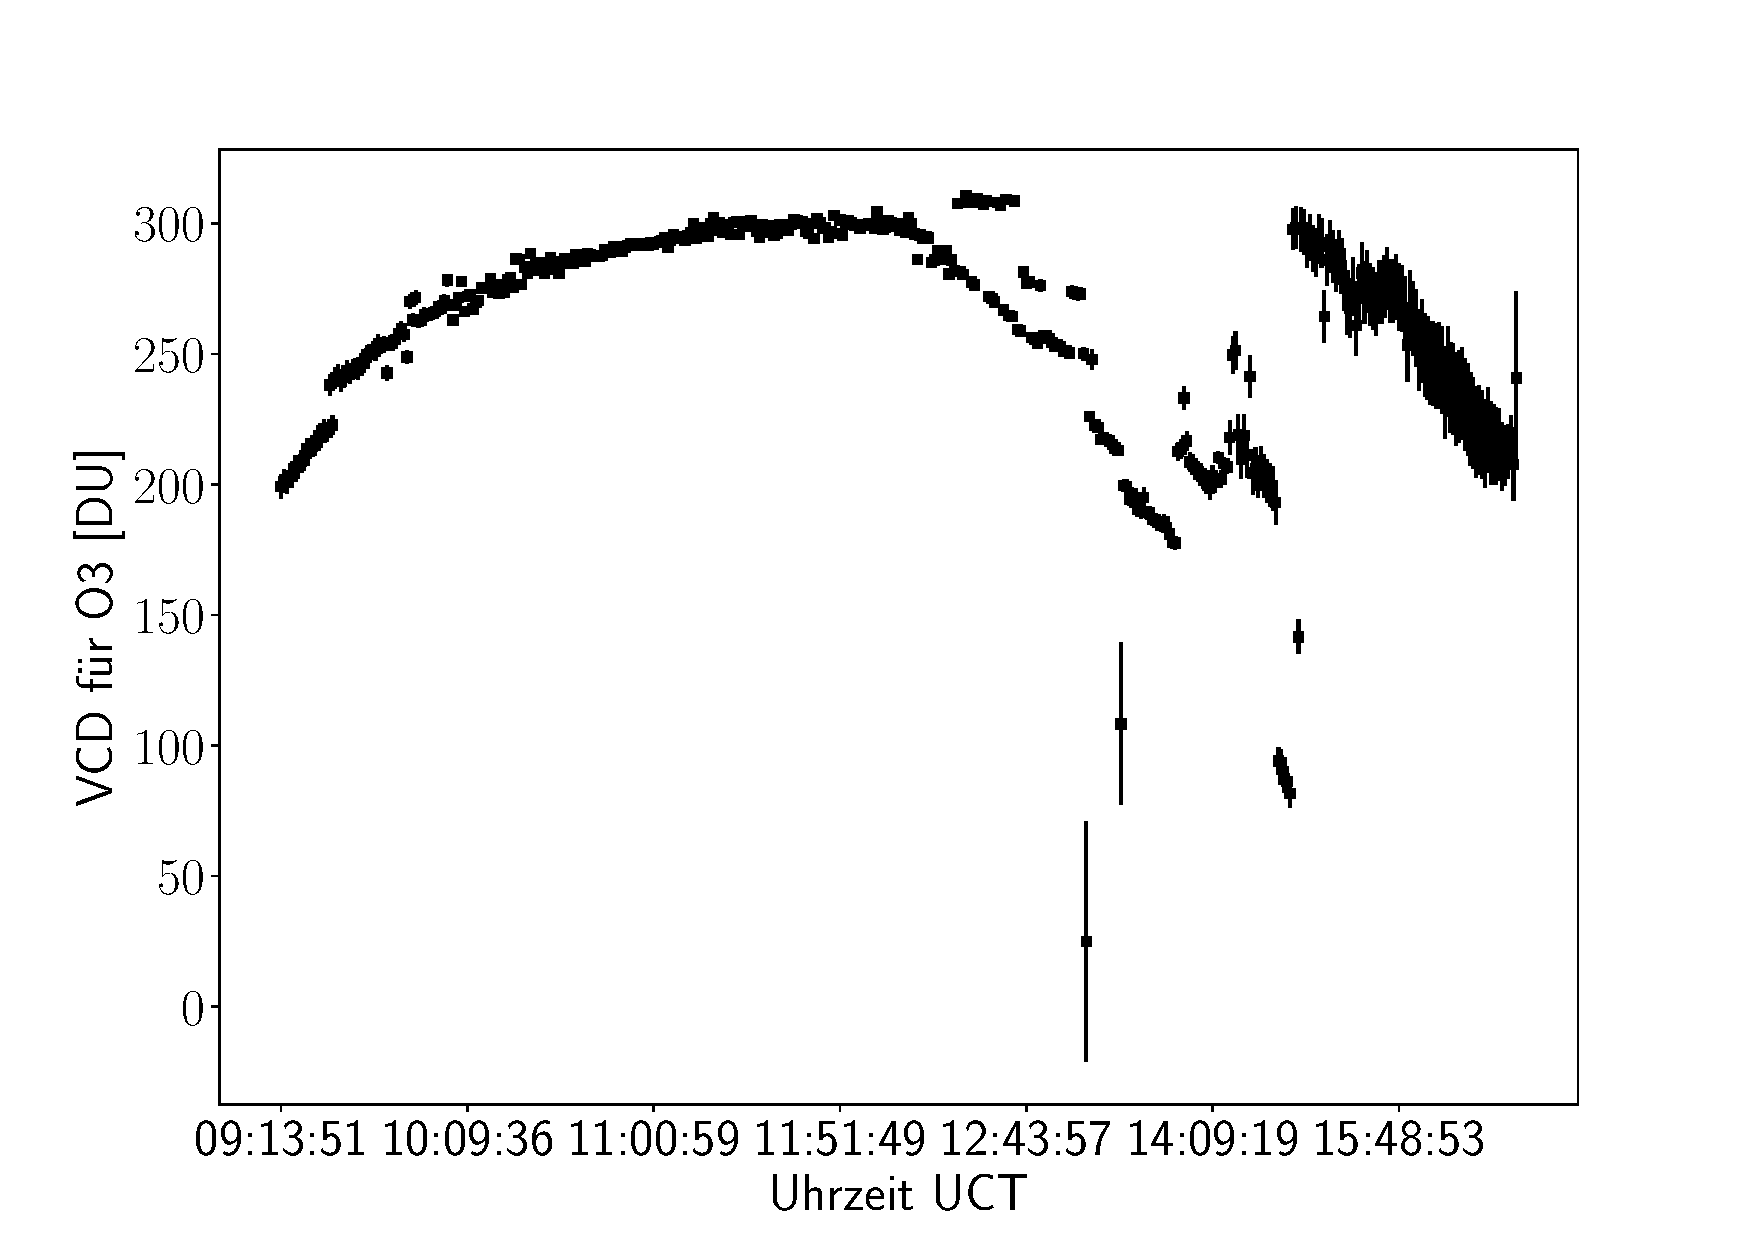
\includegraphics[width=.7\linewidth]{fig/VCD_O3_over_day.pdf}
		\caption{vertikale Säulendichte Tagesmessung \ch{O3}}    
	\end{figure}
\end{frame}

\begin{frame}
	\frametitle{Vertikale Säulendichte \ch{O3} von NASA Messungen}
	\vspace{-0.35cm}
	\begin{columns}
      \column{0.9\linewidth}	
		\begin{figure}	
    		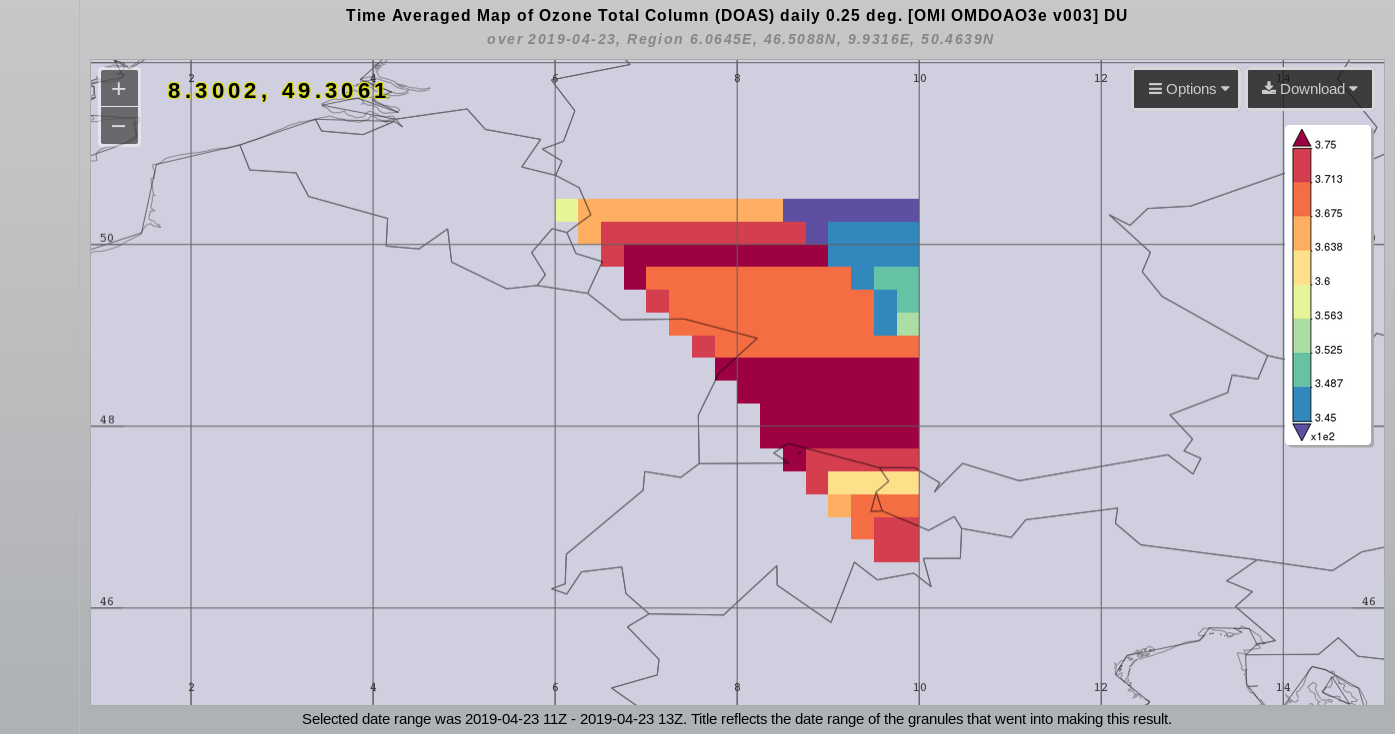
\includegraphics[width=0.65\linewidth]{fig/DOAS_VCD_Ozone_ohne_Maus.png}
    	\end{figure}
    	\vspace{-1cm}
    	\begin{figure}
    		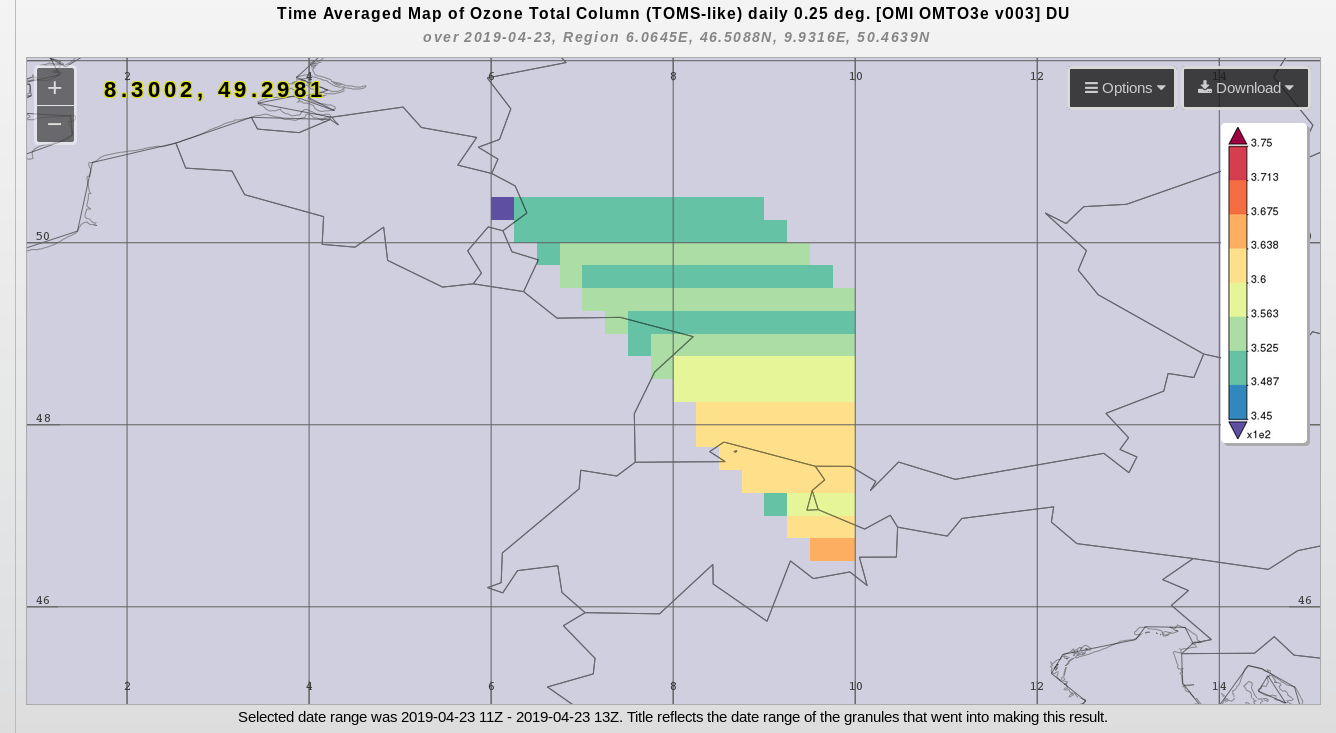
\includegraphics[width=0.65\linewidth]{fig/TOMS_VCD_Ozone_ohne_Maus.png}
    		\caption{\ch{O3} Satellitenmessungen des 23.04.2019 \cite{giovanni_nasa}}
    	\end{figure}		
	  \column{0.1\linewidth}
      	\begin{figure}	
      		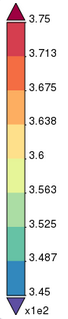
\includegraphics[width=1\linewidth]{fig/DOAS_VCD_Ozone_legende.png}
      	\end{figure}
	\end{columns}
\end{frame}

\begin{frame}
    \frametitle{Multi Axis DOAS}
    Liefert Einblick in die vertikale Verteilung der Spurengase \\
    Jetzt $\alpha$: Winkel zwischen Horizont und Richtung der Kamera
    \begin{figure}
        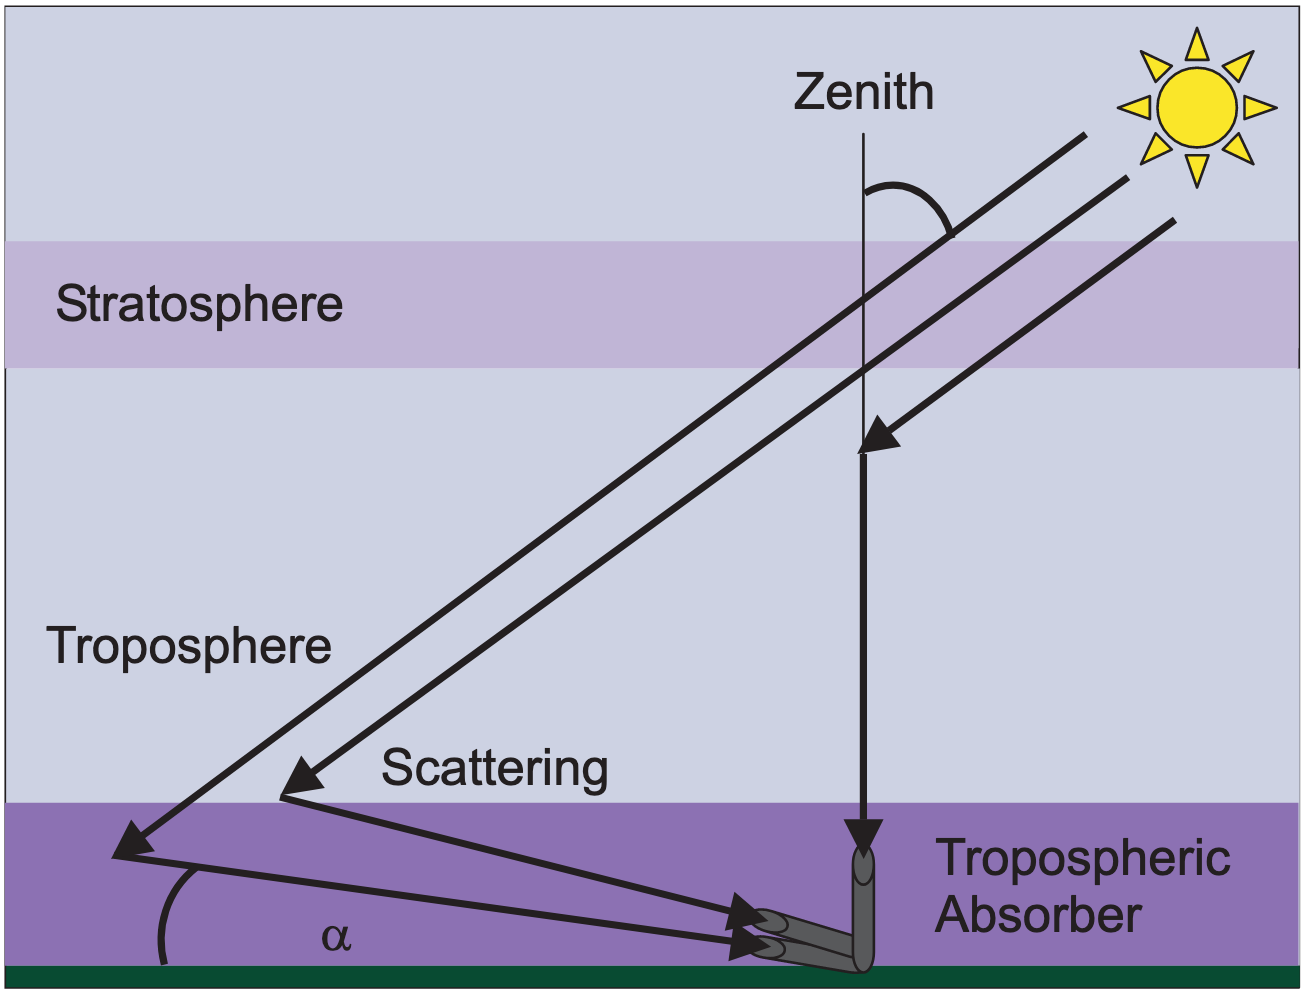
\includegraphics[width=.6\linewidth]{fig/photo/max_doas.png}
        \caption{schematischer Lichtweg bei Multi Axis DOAS Messungen \cite{atm_script}}
    \end{figure}
\end{frame}

\begin{frame}
    \frametitle{Multi Axis DOAS}
    Vier Messreihen bei jeweils $7^\circ$, $12^\circ$ und $90^\circ$ \\
    \begin{figure}
    	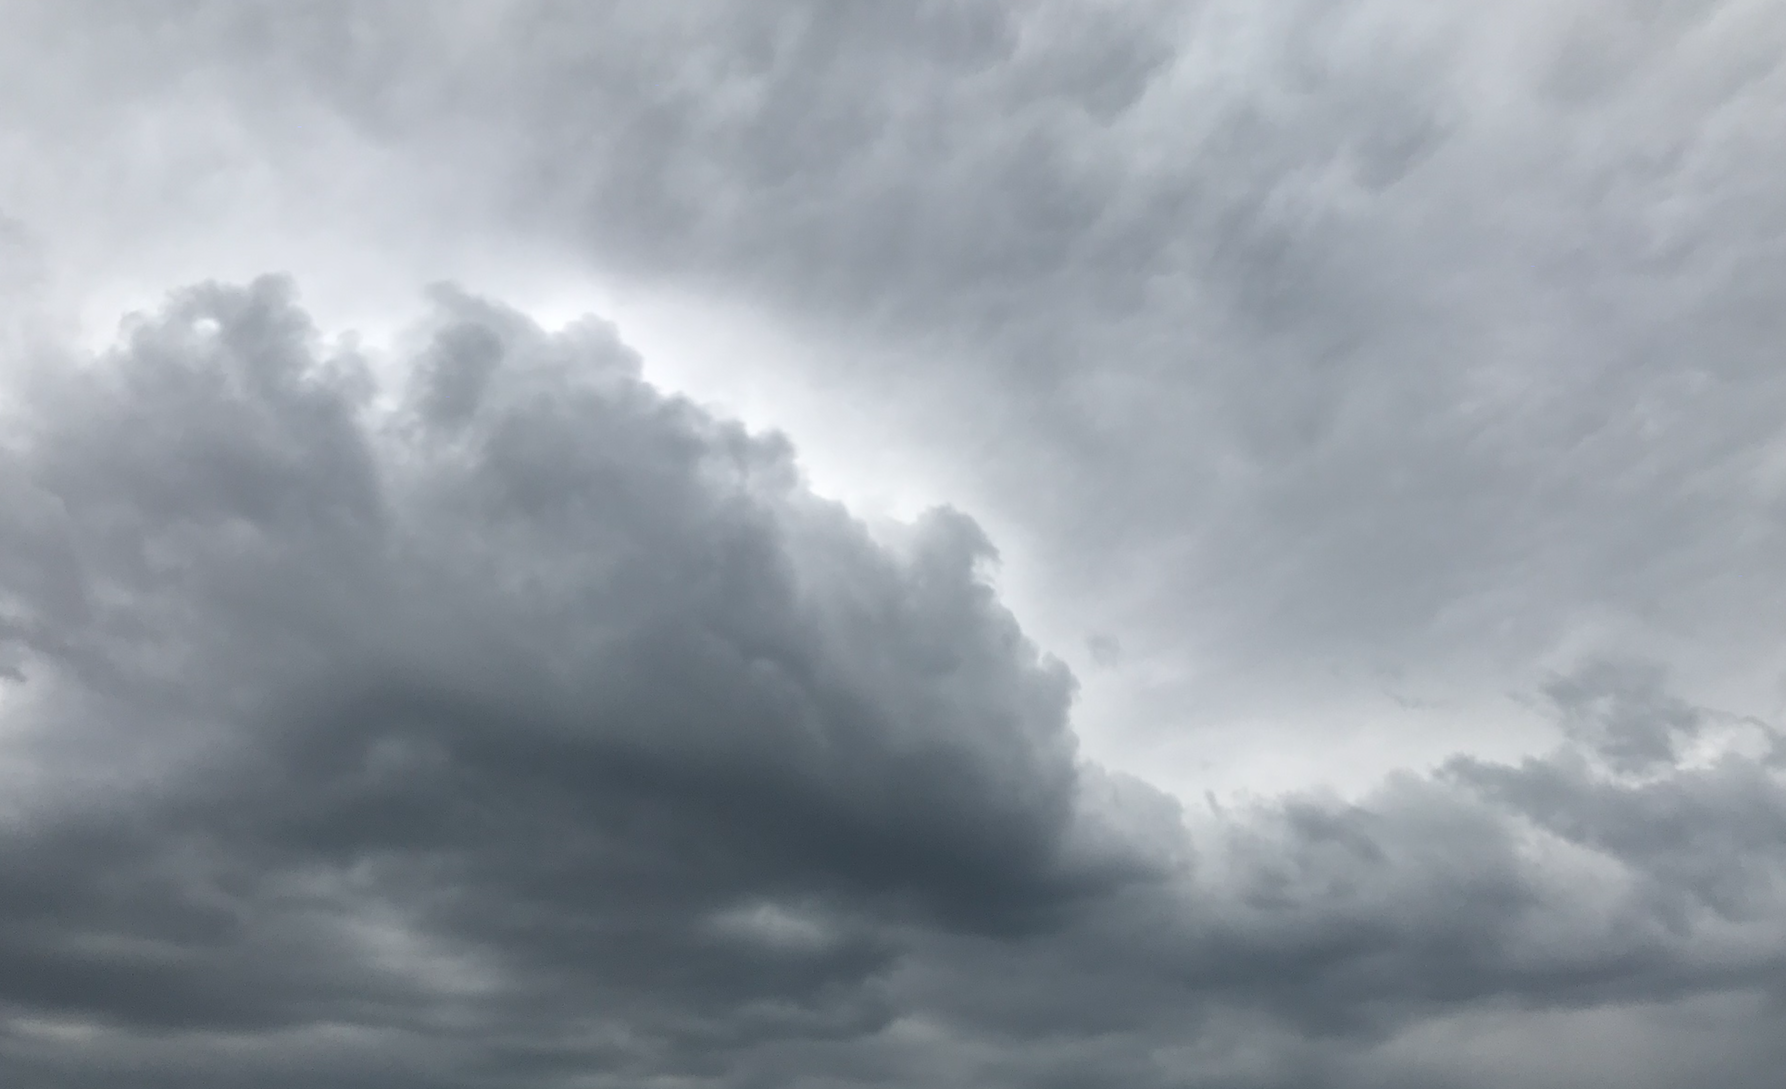
\includegraphics[width=.7\linewidth]{fig/photo/wetter.png}
    	\caption{Wetterverhältnisse am 02.05.2019}
    \end{figure}
\end{frame}

\begin{frame}
    \frametitle{MAX-DOAS Messung}
    \begin{columns}
      \column{0.5\linewidth}
    	\begin{figure}
    		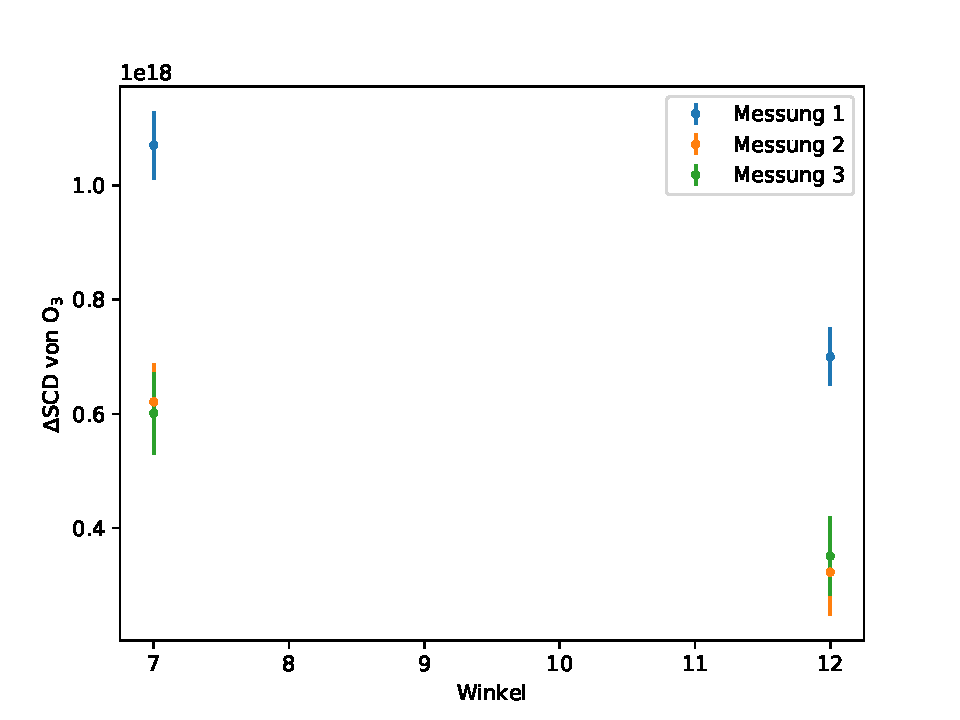
\includegraphics[width=1.2\linewidth]{fig/max_DOAS_O3.pdf}
    		\caption{Messung \ch{O3}}
    	\end{figure}
	  \column{0.5\linewidth}
	  	\begin{figure}
	  			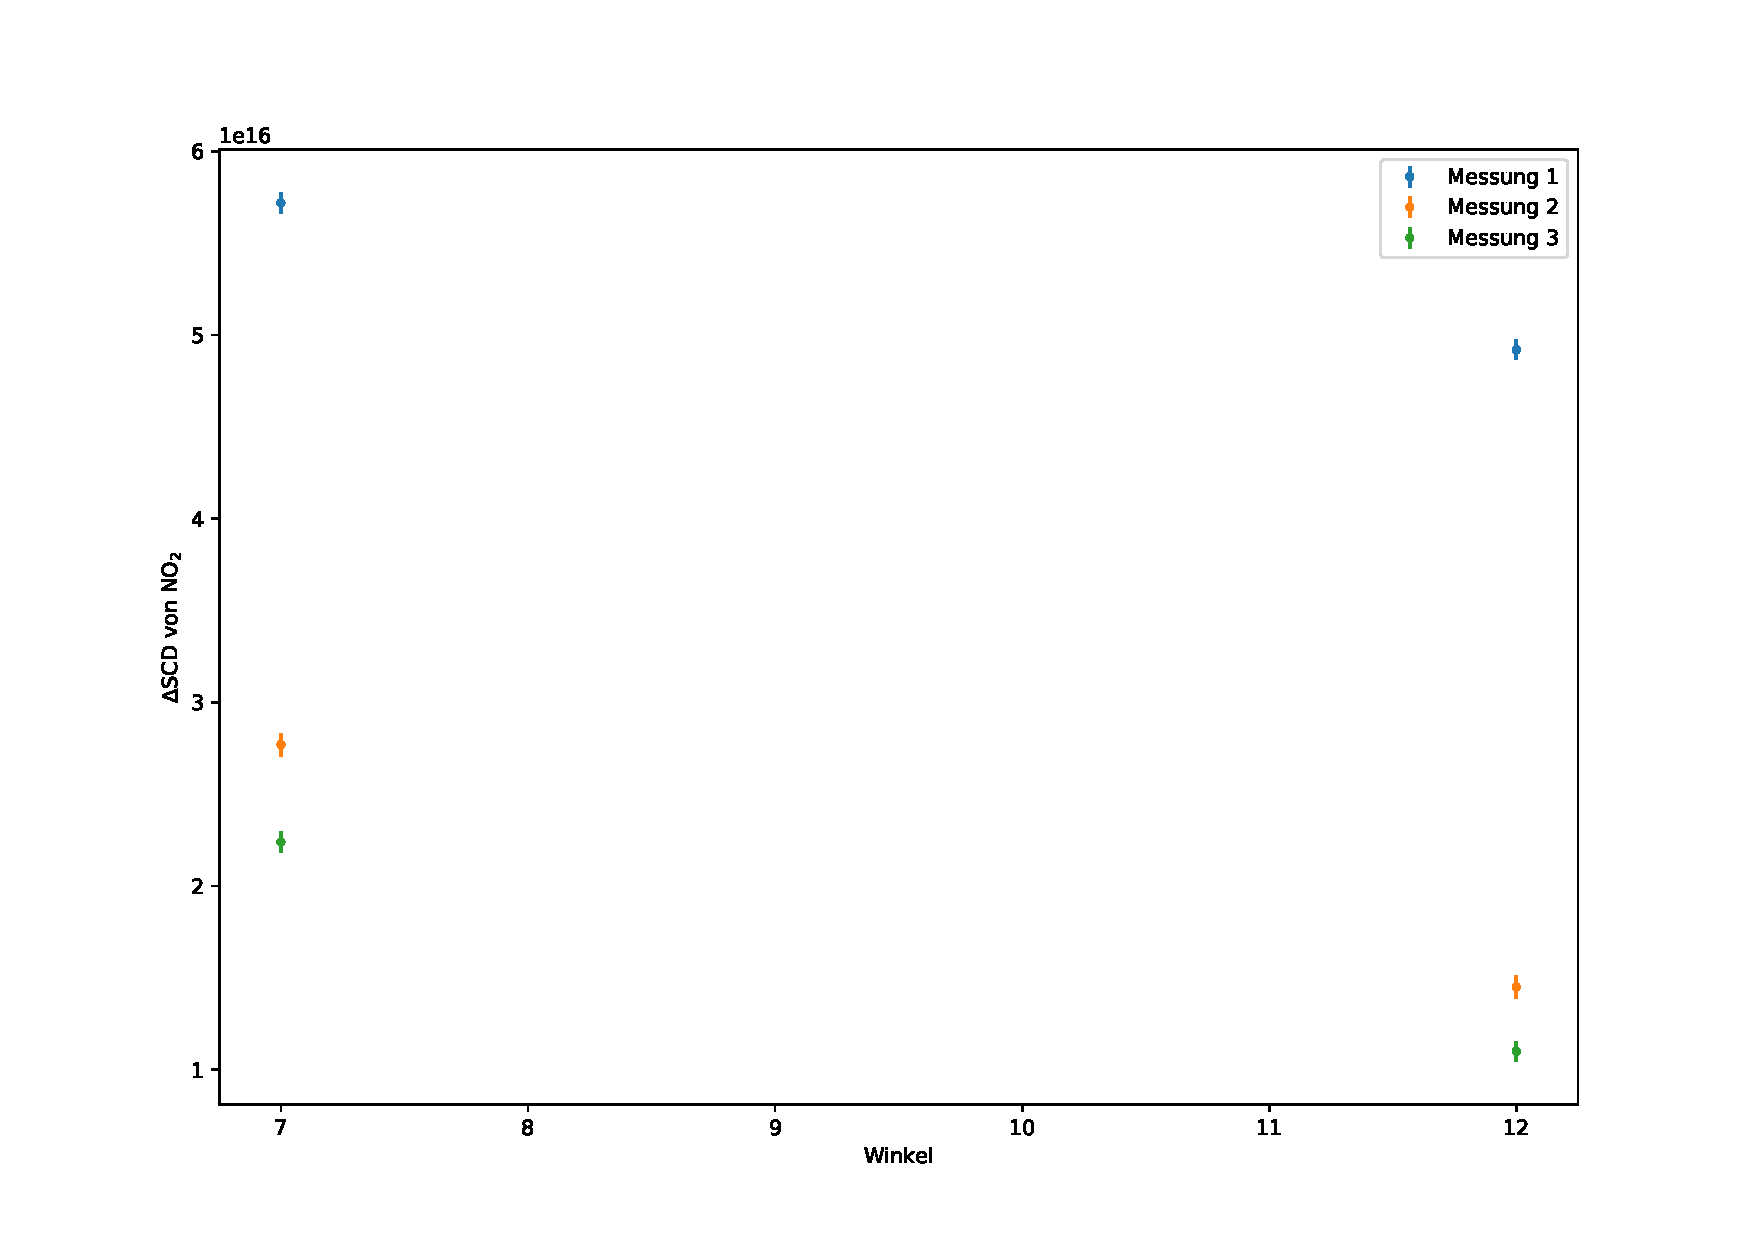
\includegraphics[width=1.2\linewidth]{fig/max_DOAS_NO2.pdf}
	  			\caption{Messung \ch{NO2}}
	  	\end{figure}
	\end{columns}
\end{frame}

\begin{frame}
	\frametitle{MAX-DOAS Messung}
	\begin{columns}
  	  \column{0.5\linewidth}    
    	\vspace{-1cm}
    	\begin{figure}
    		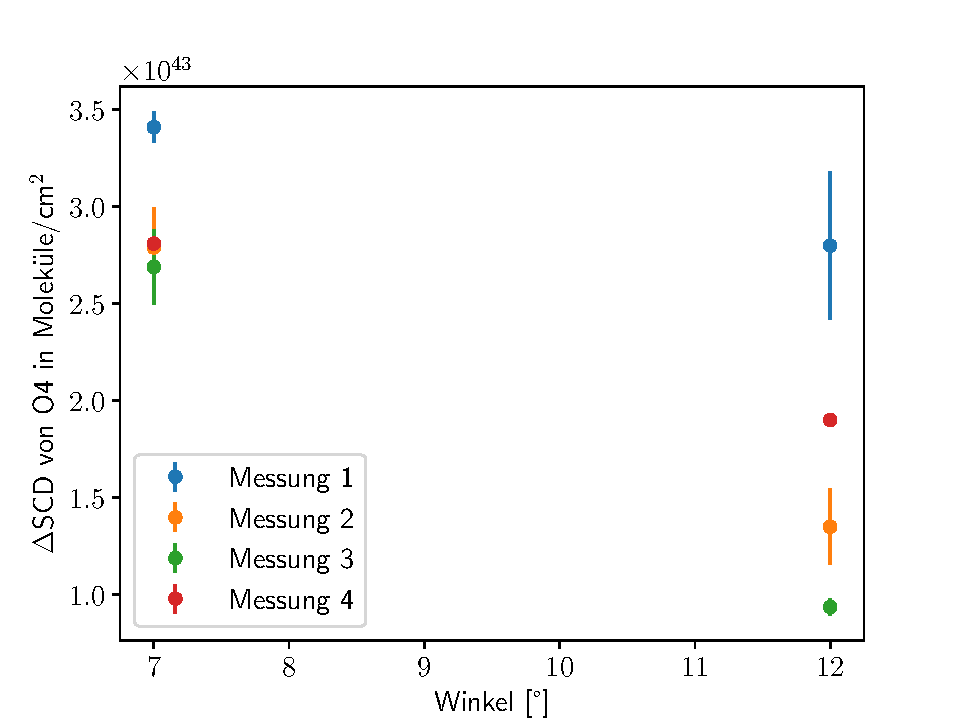
\includegraphics[width=1.2\linewidth]{fig/max_DOAS_O4.pdf}
    	\end{figure}
  	  \column{0.5\linewidth}
		\begin{center}
			\begin{tabular*}{\linewidth}{c c}
		  		\toprule
				Molekül & Verhältnis $\Delta \text{SCD}$ \\
				\midrule
				\ch{O3} & $1.0 \pm 0.4$ \\
				\ch{NO2} & $1.4 \pm 1.1$ \\
				\ch{O4} & $1.7 \pm 0.7$\\
				\bottomrule
			\end{tabular*}
			\captionof{table}{Verhältnis der $\Delta$SCD von \ch{O3}, \ch{NO2} und \ch{O4}}
			\label{fig:ratio_dscd}
		\end{center}
	\end{columns}
\end{frame}

\begin{frame}
	\frametitle{Fazit}
	\begin{itemize}
		\item[-] Konnten die Erwartungen in unseren Messungen wiederfinden  
		\pause
		\item[-] Aufgrund Näherungen werden Fehler unterschätzt
		\pause
		\item[-] Wetterverhältnisse beeinflussen die Messergebnisse
		\pause
		\item[-] Gibt guten Einblick in die Arbeit mit dem DOAS Verfahren
	\end{itemize}
\end{frame}

\begin{frame}
	\frametitle{Bildquellen}
	\linespread{0.9}
	\printbibliography
\end{frame}

\end{document}